% Part III of a082528-rounding-extinction: Periodic_Rounding_Extinction,
% added by the ProveIt write of batch 110 (7 October 2026). \input by
% questions.tex after rates.tex, before Appendix A. Labels carry the
% prefix rex:sch:.
\part{Microscopic schedules in rounding extinction: averaged ceiling laws, exact Gamma constants, discontinuous perturbations, and a sharp spectrum of limits}
\label{rex:sch:part}

\section{Provenance, scope and notation of Part III}\label{rex:sch:sec:front}

[Added 7 October 2026, batch~110.] Part~III was added in the write of
batch~110. It is built from the manuscript \emph{Microscopic Schedules in
Rounding Extinction}, which starts from Part~I's Research
question~\ref{rex:q:schedules} and answers it for a large class of weight
schedules. Everything of that manuscript is printed below: its abstract
and scope paragraph in this section, its sections as
\cref{rex:sch:sec:introduction} to \cref{rex:sch:sec:questions}, and its
two appendices, ``Proof dependencies and source audit'' and ``Notation
reference'', as the closing \cref{rex:sch:sec:audit,rex:sch:sec:notationref}
of Part~III (this report's own appendices follow Part~III). Its symbols are
kept (\cref{rex:sch:sec:notation}). Bracketed notes beginning ``[Added
7 October 2026, batch~110'' and remarks marked \textsf{[write]} are the
write's; all other text of Part~III is the manuscript's.

\subsection{The manuscript}\label{rex:sch:sec:provenance}

The manuscript is the archive \nolinkurl{Periodic_Rounding_Extinction.zip}
(1,681,098 bytes; 23 files in an inner directory
\texttt{periodic\_rounding\_extinction/}), which arrived in commit
\texttt{e4d5dcf9e}, was held from batch~114 so that this report would
receive one write, and was placed in this report by commit
\texttt{8622ca7e5} (batch~110). Its article
\texttt{periodic\_rounding\_extinction.tex} (1,901 lines; a 29-page PDF) is
titled \emph{Microscopic Schedules in Rounding Extinction}, subtitled
\emph{Averaged ceiling laws, exact Gamma constants, discontinuous
perturbations, and a sharp spectrum of limits}, and dated 5~October 2026.
Its author line and PDF author field read ``Research article prepared for
Vladimir Reshetnikov with OpenAI'', as Part~I's do; it names OpenAI as the
tool and no human author. Its pin is ProveIt commit
\texttt{52d8ca404b076c38eb7c513569592ebd8c479115} (5~October 2026), quoted
in \cref{rex:sch:sec:introduction} and in its bibliography entry for this
report. Its source audit,
\path{03-schedules-SOURCE_AUDIT.txt}, records the Git blob identities of
Part~I's \texttt{body.tex}, \texttt{extensions.tex}, \texttt{questions.tex},
\texttt{bibliography.tex} and \texttt{README.md} at the pin; the write
confirmed that all five equal the blobs at the pin and at the parent of
this write. The manuscript's statements about the repository (Part~I has
the backward-threshold method, the power-weight constant, smooth-ratio
universality and the repeated-weight example; its open problem is
Research question~\ref{rex:q:schedules}, label \texttt{rex:q:schedules})
are true. It does not know Part~II, which reached the repository later.

The manuscript cited this report twice, as its bibliography entries
\texttt{repo-report} (the report, with the pin and directory) and
\texttt{repo-questions} (its Section~10 and the label
\texttt{rex:q:schedules}). In Part~III the one sentence citing them points
to Part~I instead (\cref{rex:sch:sec:introduction}); the other citations
go to this report's bibliography, the two papers of Erd\H{o}s and
Jabotinsky to its single entry for both, and DLMF to its Chapter~5 entry
with the section the manuscript names. Figure files carry the prefix
\texttt{03-schedules-}. The uncaptioned notation table of the manuscript's
second appendix received a caption (\cref{rex:sch:tab:notationref}), so that
its PDF destination is unique, and the \texttt{latexmk} command line of
\cref{rex:sch:sec:computations} is set in a smaller font so that it fits
this report's narrower A4 text width. Labels carry the prefix
\texttt{rex:sch:}, and the ten questions of \cref{rex:sch:sec:questions}
received labels. No other text was changed.

The manuscript's abstract and its scope paragraph read as follows.

\begin{quote}\small
Starting from an integer $n$, repeatedly round down to a multiple of a
positive weight $w_k$. The power weights $w_k=k^m$ lead to OEIS A073047,
A082527, and A082528. A recent ProveIt report determines their leading
extinction constants and asks how oscillating microscopic weight changes
alter the answer. We prove a general averaging theorem for bounded local
increments whose empirical distribution converges. The necessary state
records both $\beta_k=k(w_k/w_{k-1}-1)$ and whether the increment is
strictly positive. An active increment tending to zero contributes one
integer unit to the backward dynamics; an exact repetition contributes
none. The limiting drift is an average of ceilings, and a single integral
determines the complete trajectory and extinction constant. Commensurable
positive slopes give finite Gamma products. We construct weights that
differ by less than every inverse power of their index but have different
leading constants, and weights with periodic limiting slopes for which
the constant does not exist. Bounded modifications on a set of density
zero preserve the law. Finally, at each fixed growth index $m>0$, every
constant in the sharp interval $(0,1/(m+1))$ is realized by a finite-type
schedule. A finite M\"obius inversion recovers the entire bounded
increment law from its drift. The proofs include finite enclosures for the constants, an
explanation of the losses caused by almost invisible weight changes,
and reproducible exact-arithmetic checks.

\noindent\textbf{Scope and status.}
This is a self-contained research manuscript with proofs and accompanying
computations. The periodic-schedule and bounded sparse-exception questions
of the cited repository report are resolved under the hypotheses stated
here. The classical linear asymptotic and the previously reported
power-weight Gamma constant are credited. We do not claim to settle the
classical bounded-error conjecture or to establish exhaustive historical
priority. The manuscript has not been peer reviewed or formally verified.
\end{quote}

\paragraph{Status and non-claims of the manuscript, kept.} It credits the
classical linear asymptotic, the backward-threshold method and the
power-weight Gamma constant (Erd\H{o}s--Jabotinsky; Part~I), credits
successive increment regimes to the sieve literature and discontinuous
averaging to the literature on piecewise-smooth averaging, and does ``not
claim to settle the classical bounded-error conjecture or to establish
exhaustive historical priority''; its targeted search ``does not certify
global novelty''. Its main theorem has no rate in $K$. The spectrum theorem
concerns positive real weights, allows the increment bound to depend on the
constant, and uses dormant phases; it is not claimed for integer weights
or strictly increasing schedules. The recovery theorem concerns exact data,
not stable recovery from noisy observations. Its decimal displays are
rounded, and its exact rational certificates are the stored fractions. The
manuscript ``has not been peer reviewed or formally verified''; nothing in
Part~III is formalized in Lean or Rocq. Neither the manuscript nor the
write submitted anything to OEIS.

\subsection{What Part III adds}\label{rex:sch:sec:adds}

{\small
\renewcommand{\arraystretch}{1.12}
\setlength{\LTcapwidth}{\textwidth}
\begin{longtable}{@{}>{\raggedright\arraybackslash}p{.27\textwidth}>{\raggedright\arraybackslash}p{.27\textwidth}>{\raggedright\arraybackslash}p{.38\textwidth}@{}}
\caption{The manuscript of Part~III against Parts~I and~II.}\label{rex:sch:tab:claims}\\
\toprule
Part III & Parts I and II & Status here\\
\midrule
\endfirsthead
\toprule
Part III & Parts I and II & Status here\\
\midrule
\endhead
\bottomrule
\endfoot
\Cref{rex:sch:lem:duality}, \eqref{rex:sch:eq:accounting}--\eqref{rex:sch:eq:tail-accounting} & \eqref{rex:eq:weighted-duality}, \eqref{rex:eq:weighted-error-general}--\eqref{rex:eq:weighted-tail} & same, without strict increase of the thresholds\\
\Cref{rex:sch:lem:rv} & \cref{rex:lem:regular} & the same conclusions from convergent empirical means instead of convergent ratios\\
\Cref{rex:sch:thm:main} & \cref{rex:thm:weights-main}; \cref{rex:qt:prop:profilebound} & new; the law $\delta_{(m,1)}$ gives Part~I's theorem for nondecreasing weights, and its certificate~\eqref{rex:sch:eq:certificate} is \eqref{rex:qt:eq:Phiubound} (\cref{rex:sch:rem:parts})\\
\Cref{rex:sch:thm:gamma}, \eqref{rex:sch:eq:unequal-gamma}, \cref{rex:sch:cor:one-positive} & \eqref{rex:eq:constants}, \cref{rex:prop:blocks} & new; one type gives $L_m$, and $a=0$ gives the block constant $L_m/r$\\
\Cref{rex:sch:thm:jump,rex:sch:thm:flat-perturbation,rex:sch:thm:no-limit}, \cref{rex:sch:prop:activation} & \cref{rex:sec:clock} & new: instability below every power of the index; a schedule with no limit\\
\Cref{rex:sch:thm:loss} & \cref{rex:cor:losses} & new: the loss measure marked by the increment state; its time marginal for $\delta_{(m,1)}$ is \eqref{rex:eq:loss-density}\\
\Cref{rex:sch:thm:continuity}, \cref{rex:sch:cor:sparse} & question ``Stability under sparse exceptional steps'' & new; answers its bounded form\\
\Cref{rex:sch:prop:scaling}, \cref{rex:sch:thm:spectrum} & --- & new: the constants at fixed $m$ are exactly $(0,1/(m+1))$\\
\Cref{rex:sch:prop:shape}, \cref{rex:sch:thm:recovery} & --- & new: the drift determines the law\\
\end{longtable}
}

\begin{remark}[\textsf{[write]} The one-type law is Parts~I and~II]\label{rex:sch:rem:parts}
[Added 7 October 2026, batch~110.] Let $\mu=\delta_{(m,1)}$, the law of
nondecreasing weights with $k(w_k/w_{k-1}-1)\to m$. Then $\eta=0$,
$\rho=1$, and $D(z)=C(mz)$. Since $C(mu)=\lceil mu\rceil$ for $u>0$ and
$C(0)=1$, the integrand $u+D(u)$ is Part~II's $f_p(u)$ with $p=m$, so
$H=I_m$ and $t(z)=e^{-I_m(z)}$. Hence $z=U_m(t)$ along the profile, and
\eqref{rex:sch:eq:parametric-profile} gives $y(t)=tU_m(t)=y_m(t)$ by
\cref{rex:qt:rem:identify}. The constant is
$L(\mu)=\lim_{z\to\infty}z\,e^{-(m+1)I_m(z)}=L_m$ by~\eqref{rex:qt:eq:Iasymp}
and~\eqref{rex:qt:eq:H0}, $F$ is $F_m$, and the
certificate~\eqref{rex:sch:eq:certificate}, which reads
$z\,t(z)^{m+1}\le L\le(z+1/(m+1))\,t(z)^{m+1}$, is
\eqref{rex:qt:eq:Phiubound} with $u=z$; at $z=j/m$, where $t(z)=t_j$, it is
Part~I's bracket~\eqref{rex:eq:L-brackets}. \Cref{rex:sch:thm:main} thus
contains Part~I's \cref{rex:thm:weights-main} for nondecreasing weights;
Part~I's hypothesis also admits finitely many early decreases, which
\cref{rex:sch:thm:main} excludes. The two Parts use different
normalizations of one letter: Part~I's $z(t)$ is $my(t)/t$, Part~III's
$z(t)$ in~\eqref{rex:sch:eq:z-definition} is $y(t)/t$. With that,
the time marginal of \cref{rex:sch:thm:loss} for $\delta_{(m,1)}$ has
density $t^m\bigl(C(mz)-mz\bigr)/L_m$ with Part~III's $z$, which is
Part~I's~\eqref{rex:eq:loss-density}.
\end{remark}

\paragraph{Questions of Part~I.} Research question~\ref{rex:q:schedules}
asks for the limits when $k(w_k/w_{k-1}-1)$ oscillates, has repeated zero
values or follows a periodic pattern, and which information beyond the
index determines the constant and the profile. \Cref{rex:sch:thm:main}
answers it for nondecreasing weights with uniformly bounded scaled
increments whose augmented empirical law converges: the additional
information is that law, the joint frequency of the scaled increment and of
the activity flag, through the averaged drift~$D$; the order of the steps
does not enter, and $D$ determines the law (\cref{rex:sch:thm:recovery}).
Outside that class the question stays open, re-scoped as Part~III's
questions on unbounded or signed increments
(Research question~\ref{rex:sch:q:unbounded}) and on schedules without a
limiting law (Research question~\ref{rex:sch:q:nonconv}); without a
limiting law the constant need not exist (\cref{rex:sch:thm:no-limit}).
The question ``Stability under sparse exceptional steps''
(Research question~\ref{rex:q:sparse}) is answered in its bounded form by
\cref{rex:sch:cor:sparse}: bounded changes on a set of density zero leave
the law, the constant and the profiles unchanged. Whether a sparse set of
very large jumps can change the constant stays open
(Research question~\ref{rex:sch:q:sparse}). Dated notes at Part~I's
questions say so.

\subsection{Notation of Part III}\label{rex:sch:sec:notation}

Part~III keeps the manuscript's symbols; no symbol is renamed and no
normalization is changed. It shares most of Part~I's letters with the
same meanings: $w_k$, $x_k$, $\tau_w(n)$, $T_w(K)$, $q_k^{(K)}$, $b_k$, the
positive ceiling $C$, and $m$, $L$ and $F$ in the power case
(\cref{rex:sch:rem:parts}). \Cref{rex:sch:tab:notation} lists the letters
that mean something else in Parts~I or~II.

{\small
\renewcommand{\arraystretch}{1.1}
\setlength{\LTcapwidth}{\textwidth}
\begin{longtable}{@{}>{\raggedright\arraybackslash}p{.17\textwidth}>{\raggedright\arraybackslash}p{.36\textwidth}>{\raggedright\arraybackslash}p{.39\textwidth}@{}}
\caption{Letters of Part~III that have other meanings in Parts~I
and~II.}\label{rex:sch:tab:notation}\\
\toprule
Part III & Meaning & Meaning elsewhere\\
\midrule
\endfirsthead
\toprule
Part III & Meaning & Meaning elsewhere\\
\midrule
\endhead
\bottomrule
\endfoot
$m$ & mean slope $\int\beta\,d\mu$ & Part~I: the exponent; equal for power weights\\
$L=L(\mu)$ & limit of $T_w(K)/(Kw_K)$ & Part~I: $L_m=L(\delta_{(m,1)})$; Part~II: $K_p$\\
$z(t)=y(t)/t$ & & Part~I: $z(t)=my(t)/t$\\
$\beta_k$, $\sigma_k$ & scaled increment, activity flag & Part~II: $\beta=s/(s+1)$ a cutoff exponent\\
$\mu$; $\mu_N$; $\nu_n$ & limiting law; empirical laws; marked loss measures & Part~I: $\mu_n$ are the loss measures \eqref{rex:eq:loss-measure}\\
$\rho$, $\eta$ & activity, active-zero mass & Part~I: $\rho_m$ is the loss density\\
$D(z)$, $E(z)$ & averaged drift, residual $D(z)-mz$ & Part~I: $E_m(K)$ in Research question~\ref{rex:q:rates}; Part~II: the constant $E_p$\\
$H(z)$, $t(z)$ & integral and time of the profile & Part~II: $H_p(t)$ is a mass profile; Part~I: $t_j$ are crossing times (here $t(j/m)=t_j$ for $\delta_{(m,1)}$)\\
$M(t)=t^my(t)$ & & Part~I: $f_m$; Part~II: $M_{k,j}$\\
$y(t)$ & backward profile & Part~I: $y_m$, the case $\delta_{(m,1)}$\\
$Q$; $Q_k$ & cell length $1/\lambda$; forward quotients & Part~I: $Q_k$ forward quotients; Part~II: $Q_p$ a ratio bound\\
$A_j$, $B_j$ & Gamma arguments & Part~II: $A_p(n)$, $B_p(k)$\\
$B$; $\mathcal E_B$ & increment bound; state space & Part~II: $B_p$; the denominator $B$ of $p=A/B$\\
$a$ & number (or frequency $a/r$) of active zero phases & Part~I: $a=m/(m+1)$; Part~II: $a=1/s$\\
$r$ & period length & Part~I: the block length $r$ (the same role, \cref{rex:prop:blocks})\\
$s$; $p_s$; $\alpha_s$; $h_s$ & type index; frequency; slope; integer multiple & Part~II: $s=p+1$, $p$ the exponent\\
$p$ in \cref{rex:sch:sec:computations} & length of a periodic tuple & Part~II: the exponent\\
$h_j$; $h$ in \cref{rex:sch:thm:no-limit} & perturbation sizes; block index & Part~II: terminal quotient\\
$A\subseteq\N$, $\theta$ & set of perturbed indices, its density & Part~II: $A_p(n)$\\
$c$ & thinning factor & Part~I: $c_m$\\
$R$ & cutoff in proofs & Part~II: $R_j$, $R_k$\\
$f(x)$, $G(x)$, $\mathfrak m$ & tail of the slope law, its sum, M\"obius function & Part~I: $f_m=t^my_m$\\
\end{longtable}
}

\paragraph{Intake checks.} The dossier of the intake (6~October 2026)
reran the manuscript's program on a copy with
\texttt{-{}-no-figures}: it exited normally in 41\,s; the four CSV files
were byte-identical to the recorded ones, the three JSON files equal apart
from line ends, and the console output equal to the recorded log apart
from the line reporting the figures, which that run did not regenerate. It
recomputed $T/(Kw_K)=0.1591535$ for $\varepsilon=0$ and $0.3927036$ for
$\varepsilon=10^{-4}$ at $K=10^5$ (\cref{rex:sch:tab:epsilon}), and found
the two-phase constant~\eqref{rex:sch:eq:unequal-gamma} inside its own
finite certificate $[0.33185619,0.33193915]$ at $z=2000$. The write
evaluated the Gamma products to forty digits: the two-phase constant is
$0.33189767362899860\ldots$, the three-phase constant of
\cref{rex:sch:tab:positive} is $0.32927650881086035\ldots$, and the
expansion in~\eqref{rex:sch:eq:Lr-gamma} holds, the remainder times $r^2$
being $0.0625$ for $m=1$ and $0.0278$ for $m=2$ at $r=1000$.

\section{The OEIS problem and the new questions}
\label{rex:sch:sec:introduction}

For positive weights $w_1=1,w_2,w_3,\ldots$, define
\begin{equation}\label{rex:sch:eq:forward}
 x_1=n,\qquad x_k=w_k\floor{\frac{x_{k-1}}{w_k}}\quad(k\geq2),
 \qquad \tau_w(n)=\min\{k\geq1:x_k=0\}.
\end{equation}
Here $n$ is a nonnegative integer, and $\tau_w(0)=1$. Intermediate values
may be real, although $x_k/w_k$ is always an integer. Every step removes
a nonnegative amount. If $w_k\to\infty$, extinction occurs in finite time.

The choices $w_k=k,k^2,k^3$ are respectively \OEIS{A073047},
\OEIS{A082527}, and \OEIS{A082528}. The cubic entry records Cloitre's
question about a leading equivalent for general real $m>0$
\cite{oeis-linear,oeis-square,oeis-cube}. The associated least initial
value surviving through stage $K$ is
\begin{equation}\label{rex:sch:eq:threshold-definition}
 T_w(K)=\min\{n\in\N:\tau_w(n)>K\}.
\end{equation}
For $w_k=k$, this is the classical Tchoukaillon threshold sequence
\OEIS{A002491}. Erd\H{o}s and Jabotinsky proved
$T_w(K)=K^2/\pi+O(K^{4/3})$ \cite{erdos-jabotinsky}.

The ProveIt report \emph{Gamma Constants and Scaling Limits for Rounding
Extinction} establishes the fixed-$m$ power-weight formula
\begin{equation}\label{rex:sch:eq:old-constant}
 L_m=\frac{1}{m\Gamma(m/(m+1))^{m+1}},\qquad
 T_{k^m}(K)\sim L_mK^{m+1},
\end{equation}
and extends it to weights with $k(w_k/w_{k-1}-1)\to m$. Its microscopic
schedule question explicitly asks what happens when those local ratios
oscillate, vanish repeatedly, or have a periodic pattern
(Part~I of this report: \cref{rex:thm:weights-main} and Research
question~\ref{rex:q:schedules}). We take that question as the starting
point, and recover \eqref{rex:sch:eq:old-constant} as a specialization of the
theory below.

\subsection{What the article establishes}

The new results concern the dependence on a schedule, rather than a new
proof of the classical constant in isolation.

\begin{enumerate}
 \item \textbf{An empirical-distribution theorem.} A bounded local
 increment law, augmented by a binary activity flag, determines a
 unique backward profile, the leading threshold constant, the
 stopping-time equivalent, and the full normalized forward trajectory.
 Periodic patterns are a finite-support case; arbitrary deterministic
 schedules with convergent empirical distributions are included.
 \item \textbf{Exact constants.} Every finite pattern of commensurable
 positive slopes has a finite Gamma-product expression. Weakly active
 zero slopes contribute an explicit additive term to the drift.
 \item \textbf{A sharp instability.} For
 $w_{2j-1}=j$ and $w_{2j}=j+\varepsilon/j$, the normalized threshold
 constant is $1/(2\pi)$ at $\varepsilon=0$, and $\pi/8$ at every
 $0<\varepsilon<1$. The relative factor is $\pi^2/4$.
 The perturbation can instead be smaller than every inverse power.
 \item \textbf{Failure of a limit.} Even the same periodic limiting
 slopes and the same leading weights $w_k\sim k/2$ can coexist with
 two distinct subsequential threshold constants.
 \item \textbf{Stability and a complete range of constants.} Bounded
 changes on a density-zero set do not alter the normalized law.
 For fixed $m>0$, the set of constants over the stated class of
 schedules is exactly $(0,1/(m+1))$.
 \item \textbf{Exact inverse recovery.} The limiting drift determines
 the entire bounded augmented increment law by a finite M\"obius
 inversion. The normalized forward shape determines it up to an
 explicitly characterized drift scaling.
\end{enumerate}

\subsection{Attribution and the inspected repository}

The source audit is pinned to the repository revision
\begin{center}\small
\texttt{52d8ca404b076c38eb7c513569592ebd8c479115}.
\end{center}
The inspected directory is
\begin{quote}\small\ttfamily
SetTheory/Cardinals/docs/reports/\\
generating-functions-and-asymptotics/\\
oeis-sequence-asymptotics/a082528-rounding-extinction/.
\end{quote}
The source files \texttt{body.tex}, \texttt{extensions.tex}, and
\texttt{questions.tex} were read, and their Git blob identities were
checked against that revision. The existing report already contains the
backward-threshold method, the smooth power law, and repeated-weight
examples. The distributional averaging theorem, the general finite
Gamma product, and the instability and spectrum results below are
extensions developed here. The present proofs do not require accepting
an unproved claim in the repository.

Successive integer-increment regimes and product limits go back to the
classical sieve literature \cite{erdos-jabotinsky}. Discontinuous averaging is also
an established subject \cite{averaging}. Our assertion of contribution
is specific to the theorem, hypotheses, constants, and counterexamples
for \eqref{rex:sch:eq:forward}; it is not a claim to have invented averaging.
A targeted search did not identify the same schedule theorem in the
primary sources examined. That search does not certify global novelty.

\section{Exact survival duality and rounding-error accounting}
\label{rex:sch:sec:duality}

The forward process repeatedly discards information. Reversing the
survival condition produces an exact integer recurrence with a useful
one-sided error estimate.

\begin{lemma}[Backward thresholds]\label{rex:sch:lem:duality}
For a fixed horizon $K$, define
\begin{equation}\label{rex:sch:eq:backward}
 q_K^{(K)}=1,\qquad
 q_{k-1}^{(K)}=\ceil{\frac{w_k}{w_{k-1}}q_k^{(K)}}
 \quad(k=K,K-1,\ldots,2).
\end{equation}
Then $T_w(K)=q_1^{(K)}$. More generally, an integer quotient $Q$ at stage
$k$ survives through $K$ if and only if $Q\geq q_k^{(K)}$.
Consequently,
\begin{equation}\label{rex:sch:eq:inverse}
 \tau_w(n)>K\ \Longleftrightarrow\ n\geq T_w(K),\qquad
\tau_w(n)=J\ \Longleftrightarrow\ T_w(J-1)\leq n<T_w(J).
\end{equation}
The second equivalence is stated for $n>0$ and $J\geq2$.
\end{lemma}

\begin{proof}
At the terminal stage, survival means quotient at least one. If the
least surviving quotient at stage $k$ is $q_k$, then an input
$w_{k-1}Q$ survives precisely when
\[
 \floor{\frac{w_{k-1}Q}{w_k}}\geq q_k,
 \quad\text{equivalently}\quad
 Q\geq\frac{w_kq_k}{w_{k-1}}.
\]
Taking the least integer $Q$ gives \eqref{rex:sch:eq:backward}. Backward
induction reaches stage one, where $w_1=1$ and the initial values are
integers. The inverse statements follow directly.
\end{proof}

The thresholds are nondecreasing in $K$. They need not be strictly
increasing when some weights are repeated; no strictness will be used.
If $w_K\to\infty$, they are unbounded because a surviving initial value
is at least $w_K$.

Suppress the superscript $K$, and write $b_k=w_k/w_{k-1}-1$. The
integrality of $q_k$ gives
\begin{equation}\label{rex:sch:eq:integer-increment}
 q_{k-1}-q_k=\ceil{b_kq_k}.
\end{equation}
The original ceiling also gives the exact accounting inequality
\begin{equation}\label{rex:sch:eq:accounting}
 0\leq w_{k-1}q_{k-1}-w_kq_k<w_{k-1}.
\end{equation}
Summing it yields both of the estimates used throughout the paper:
\begin{align}
 w_kq_k&\leq w_K+\sum_{j=k}^{K-1}w_j,
 \label{rex:sch:eq:global-accounting}\\
 0\leq T_w(K)-w_kq_k&<\sum_{j=1}^{k-1}w_j\quad(k\geq2).
 \label{rex:sch:eq:tail-accounting}
\end{align}
At $k=1$ the latter difference is zero. Thus the entire initial segment
of the reversed process has a controlled weighted cost. No hypothesis
about equidistribution of fractional parts is involved.

\section{The local increment law and the main theorem}
\label{rex:sch:sec:main}

Assume from now on that the weights are nondecreasing. Define
\begin{equation}\label{rex:sch:eq:environment}
 \beta_k=k\left(\frac{w_k}{w_{k-1}}-1\right),\qquad
 \sigma_k=\ind_{\{w_k>w_{k-1}\}}\quad(k\geq2).
\end{equation}
The number $\beta_k$ measures the local relative change on its natural
$1/k$ scale. The flag $\sigma_k$ records whether a change occurs at all.

For some finite $B$, suppose $0\leq\beta_k\leq B$. The compact state
space relevant to limits is
\begin{equation}\label{rex:sch:eq:state-space}
 \mathcal E_B=\{(0,0)\}\ \cup\ ([0,B]\times\{1\}).
\end{equation}
Although a finite-stage pair cannot equal $(0,1)$, that point can be a
limit of positive increments tending to zero. It is deliberately
distinct from $(0,0)$.

\begin{definition}[Convergent increment law]\label{rex:sch:def:law}
The schedule has limiting law $\mu$ if the empirical probability
measures satisfy
\begin{equation}\label{rex:sch:eq:empirical}
 \mu_N=\frac{1}{N-1}\sum_{k=2}^{N}\delta_{(\beta_k,\sigma_k)}
 \weak\mu
 \quad(N\to\infty)
\end{equation}
weakly on $\mathcal E_B$. Set
\begin{equation}\label{rex:sch:eq:m-rho-eta}
 m=\int\beta\dd\mu,\qquad
 \rho=\int\sigma\dd\mu,\qquad
 \eta=\mu(\{(0,1)\}),
\end{equation}
and assume $m>0$. Here $\rho$ is the asymptotic fraction of active
steps, while $\eta$ is the mass of active steps whose scaled increments
vanish in the limiting law.
\end{definition}

Weak convergence means convergence of integrals of continuous functions.
For a finite set of limiting phase types it reduces to convergence of
their frequencies. No randomness is required.

Use the positive ceiling
\begin{equation}\label{rex:sch:eq:positive-ceiling}
 C(u)=\max\{1,\lceil u\rceil\}\quad(u\geq0),
\end{equation}
and define
\begin{align}
 D(z)&=\int_{\mathcal E_B}\sigma C(\beta z)\dd\mu(\beta,\sigma),
 \label{rex:sch:eq:drift}\\
 H(z)&=\int_0^z\frac{\dd u}{u+D(u)},\qquad t(z)=e^{-H(z)}.
 \label{rex:sch:eq:H}
\end{align}
These are ordinary Lebesgue integrals. Changing the values assigned at
positive-integer ceiling jumps may change $D$ at a countable set of
$z$-values, but leaves $H$, the profiles, and their integral formulas
unchanged. The convention $C(0)=1$ remains fixed. Notice the order in
\eqref{rex:sch:eq:drift}: apply the ceiling to each local type, then average.

\begin{theorem}[Averaged extinction law]\label{rex:sch:thm:main}
Under \cref{rex:sch:def:law}, the weights are regularly varying with index $m$:
\begin{equation}\label{rex:sch:eq:rv-main}
 \frac{w_{\lfloor Kt\rfloor}}{w_K}\longrightarrow t^m
 \quad\text{locally uniformly for }t>0.
\end{equation}
The function $t(z)$ decreases continuously from $1$ to $0$. It defines
a unique profile by
\begin{equation}\label{rex:sch:eq:parametric-profile}
 y(t(z))=z\,t(z),\qquad y(1)=0.
\end{equation}
The limit
\begin{equation}\label{rex:sch:eq:L}
 L=L(\mu)=\lim_{z\to\infty}z\,t(z)^{m+1}
\end{equation}
exists, is positive, and has the strict bounds
\begin{equation}\label{rex:sch:eq:universal-bounds}
 \frac{\eta}{m+1}<L<\frac{\rho}{m+1}\leq\frac{1}{m+1}.
\end{equation}
The following conclusions hold:
\begin{align}
 \frac{q_{\lfloor Kt\rfloor}^{(K)}}{K}&\longrightarrow y(t)
 &&\text{locally uniformly on }(0,1],\label{rex:sch:eq:q-limit}\\
 T_w(K)&\sim L K w_K,\label{rex:sch:eq:T-limit}\\
 n&\sim L\tau_w(n)w_{\tau_w(n)}.
 \label{rex:sch:eq:tau-limit}
\end{align}
For $J=\tau_w(n)$, the entire forward trajectory satisfies
\begin{equation}\label{rex:sch:eq:F-limit}
 \sup_{0\leq t\leq1}
 \left|\frac{x_{\max(1,\lfloor Jt\rfloor)}}{n}-F(t)\right|
 \longrightarrow0,
 \qquad F(t)=\frac{t^m y(t)}{L},\quad F(0)=1.
\end{equation}
Finally, every finite $z\geq0$ gives the certified enclosure
\begin{equation}\label{rex:sch:eq:certificate}
 \left(z+\frac{\eta}{m+1}\right)t(z)^{m+1}
 \leq L\leq
 \left(z+\frac{\rho}{m+1}\right)t(z)^{m+1}.
\end{equation}
\end{theorem}

The interpolated version of \eqref{rex:sch:eq:q-limit} and its floor-indexed
version differ by $O_\delta(1/K)$ on every $[\delta,1]$. We use either
without changing the limiting assertion.

The theorem identifies the leading term and the limiting shape. The
mere convergence in \eqref{rex:sch:eq:empirical} can be arbitrarily slow; no
numerical rate in $K$ is part of its conclusion.

\begin{corollary}[Finite phase patterns]\label{rex:sch:cor:finite-types}
Let $s_k$ take values in a finite set $S$, with
$\#\{k\leq N:s_k=s\}/N\to p_s$. For each type fix $\alpha_s\geq0$
and an activity flag $e_s\in\{0,1\}$, with $\alpha_s>0$ implying
$e_s=1$. Suppose
\[
 \beta_k-\alpha_{s_k}\longrightarrow0,\qquad
 \sigma_k=e_{s_k}\quad\text{eventually}.
\]
Then \cref{rex:sch:thm:main} applies with
\begin{equation}\label{rex:sch:eq:finite-drift}
 \mu=\sum_s p_s\delta_{(\alpha_s,e_s)},\quad
 m=\sum_s p_s\alpha_s,\quad
 D(z)=\sum_s p_s e_s C(\alpha_s z),
\end{equation}
provided $m>0$. In particular, a periodic pattern of length $r$ has
$p_s=1/r$ when its phases are listed separately.
\end{corollary}

For a zero slope there are two possibilities: exact plateau phases
have $e_s=0$, and phases with positive $o(1/k)$ relative growth have
$e_s=1$. The numerical slopes alone do not specify the theorem's input.

\section{Proof of the averaged profile theorem}
\label{rex:sch:sec:proof-profile}

We give the averaging argument in detail because ordinary pointwise
convergence of the discrete slopes is false for a periodic schedule.
The averaging must also cross the ceiling discontinuities and select
the nonzero solution at the terminal endpoint.

\subsection{Regular variation from empirical means}

\begin{lemma}[Weight ratios and small-time sums]\label{rex:sch:lem:rv}
Under the hypotheses of \cref{rex:sch:thm:main}, $w_K\to\infty$ and
\eqref{rex:sch:eq:rv-main} holds. For every $0<\delta\leq1$,
\begin{equation}\label{rex:sch:eq:weight-sum}
 \frac{1}{K w_K}\sum_{1\leq j<\delta K}w_j
 \longrightarrow\frac{\delta^{m+1}}{m+1}.
\end{equation}
\end{lemma}

\begin{proof}
The function $(\beta,\sigma)\mapsto\beta$ is continuous and bounded,
so $A(N)=\sum_{k=2}^N(\beta_k-m)=o(N)$. Also, uniformly in $k$,
\[
 \log\frac{w_k}{w_{k-1}}
 =\log(1+\beta_k/k)=\frac{\beta_k}{k}+O_B(k^{-2}).
\]
Abel summation of $(\beta_k-m)/k$ over $a<k\leq b$ expresses its
sum as endpoint terms $A(b)/b-A(a)/a$ plus a sum bounded by a constant
times $\sum_{k=a}^{b-1}|A(k)|/k^2$. Therefore that sum is $o(1)$
uniformly when $\delta K\leq a\leq b\leq M K$, for fixed positive
$\delta,M$. Adding the harmonic sum of $m/k$ proves the locally
uniform ratio limit.

For completeness the same argument controls the singular endpoint.
Given $0<\varepsilon<m$, choose a sufficiently small $\varepsilon'>0$
so that $|A(j)|\leq\varepsilon'j$ for large $j$. Abel summation then
bounds the centered harmonic sum over any $j<k\leq K$ by
$2\varepsilon'+\varepsilon'\log(K/j)$, up to a fixed initial constant.
The $O(k^{-2})$ remainder is summable. Enlarging a constant if necessary
gives
\begin{equation}\label{rex:sch:eq:potter}
 \frac{w_j}{w_K}\leq C_\varepsilon
 \left(\frac{j}{K}\right)^{m-\varepsilon}
 \quad(1\leq j\leq K).
\end{equation}
The same harmonic estimates show $w_K\to\infty$.
On $[a,\delta]$ with $a>0$, the ratio limit yields the Riemann-sum
limit $\int_a^\delta t^m\dd t$. Bound \eqref{rex:sch:eq:potter} makes the
omitted sum below $aK$ uniformly tend to zero as $a\downarrow0$.
This proves \eqref{rex:sch:eq:weight-sum}.
\end{proof}

\subsection{Compactness and terminal selection}

Interpolate the points $y_K(k/K)=q_k^{(K)}/K$ linearly. On a fixed
$[\delta,1]$, \eqref{rex:sch:eq:global-accounting}, monotonicity of the
weights, and \cref{rex:sch:lem:rv} give $q_k/K=O_\delta(1)$. Its discrete
increments obey
\begin{equation}\label{rex:sch:eq:slope-bound}
 0\leq q_{k-1}-q_k=\ceil{\frac{\beta_kq_k}{k}}
 \leq\frac{Bq_k}{k}+1=O_\delta(1).
\end{equation}
The interpolants are consequently uniformly bounded and uniformly
Lipschitz there. Arzel\`a--Ascoli and a diagonal extraction yield a
locally uniform subsequential limit $y$ on $(0,1]$, with $y(1)=0$.

At every active step, the argument of the ceiling is strictly positive,
so the increment is at least one. Hence
\[
 q_{k-1}-q_k\geq\sigma_k.
\]
Since the empirical activity frequency tends to $\rho$, summing over
an interval of indices and passing to the limit gives
\begin{equation}\label{rex:sch:eq:positive-selection}
 y(s)-y(t)\geq\rho(t-s)\quad(0<s<t\leq1).
\end{equation}
In particular, $\rho>0$, $y(t)\geq\rho(1-t)$, and
\begin{equation}\label{rex:sch:eq:z-definition}
 z(t)=\frac{y(t)}{t}
\end{equation}
is continuous and strictly decreasing on $(0,1]$. Indeed,
\[
 \frac{y(s)}s-\frac{y(t)}t
 =\frac{y(s)-y(t)}s+y(t)\left(\frac1s-\frac1t\right)>0.
\]
It runs from infinity to zero. The lower bound in
\eqref{rex:sch:eq:positive-selection} prevents an artificial interval on which
the terminal solution remains identically zero.

\subsection{Why the ceilings can be averaged}

\begin{lemma}[Joint empirical averaging]\label{rex:sch:lem:joint}
For each $0<\delta<1$, the finite measures
\begin{equation}\label{rex:sch:eq:joint-empirical}
 \frac1K\sum_{\delta K\leq k\leq K}
 \delta_{(k/K,\beta_k,\sigma_k)}
 \weak\ind_{[\delta,1]}(t)\dd t\,\mu(\dd\beta,\dd\sigma).
\end{equation}
Along a subsequence for which $y_K\to y$ locally uniformly,
the corresponding integrated ceiling increments converge to
$\int D(y(t)/t)\dd t$ on every compact time interval.
\end{lemma}

\begin{proof}
For a continuous function $g$ on $\mathcal E_B$, convergence of its
prefix averages implies
\[
 \frac1K\sum_{aK<k\leq bK}g(\beta_k,\sigma_k)
 \longrightarrow(b-a)\int g\dd\mu
\]
for fixed $0\leq a<b\leq1$. Approximating a continuous function of
$t$ by interval-step functions proves \eqref{rex:sch:eq:joint-empirical},
first for products and then for arbitrary continuous functions by
uniform approximation on the compact product space.

The ceiling integrand is
$h(t,\beta,\sigma)=\sigma C(\beta z(t))$. It is bounded on the
compact time interval. Its discontinuities can occur only when
$\sigma=1$, $\beta>0$, and $\beta z(t)$ is a positive integer.
For every fixed $\beta>0$, the strict monotonicity of $z$ makes this
a finite set of times on a compact interval. For $\beta=0$, $C(0)=1$
is continuous from the right, and the two values of $\sigma$ belong
to separate components of the state space. Fubini's theorem thus
shows that the discontinuity set of $h$ has zero measure for the
product limit in \eqref{rex:sch:eq:joint-empirical}. The usual bounded
almost-everywhere-continuous form of weak convergence therefore
applies to $h$.

There is also a moving argument: the discrete increment uses
$z_K(k/K)=q_k/k$, not $z(k/K)$. Uniform convergence of $z_K$ on the
compact interval resolves it as follows. Outside a small closed
neighborhood of the finitely many integer levels in the bounded
range of $\beta z$, the ceilings are eventually identical. The
limiting product measure of these neighborhoods tends to zero as
their width decreases, by the preceding zero-measure assertion.
Weak convergence bounds their empirical masses by arbitrarily
small numbers after choosing a slightly larger closed neighborhood.
On the omitted set the ceiling is uniformly bounded. Thus replacing
$z_K$ by $z$ changes the average by $o(1)$.

Equivalently, one can squeeze the moving ceiling between the ceilings
at $z(t)-\varepsilon$ and $z(t)+\varepsilon$ on intervals bounded
away from $t=1$, then let $\varepsilon\downarrow0$. The final
short interval near $1$ has uniformly bounded slopes and can be
removed first. Both arguments yield the stated integrated limit.
\end{proof}

The preceding proof uses a zero-measure set in the joint state space.
It does not presume that the individual periodic slopes converge at
each fixed time.

By \eqref{rex:sch:eq:integer-increment} and the definition of $C$, the slope
of $y_K$ on its $k$th interpolation interval is
$-\sigma_k C(\beta_kq_k/k)$. Integrating and applying
\cref{rex:sch:lem:joint} gives
\begin{equation}\label{rex:sch:eq:ode}
 y(t)=\int_t^1D(y(s)/s)\dd s,
 \qquad y'(t)=-D(y(t)/t)\quad\text{a.e.}
\end{equation}

\subsection{Solving the limiting equation}

The drift is nondecreasing and locally bounded. More precisely,
\begin{equation}\label{rex:sch:eq:drift-bounds}
 D(z)\geq\rho,\qquad
 \eta\leq E(z):=D(z)-mz\leq\rho\quad(z\geq0).
\end{equation}
For $z>0$ the upper inequality is strict, since positive slopes have
$\lceil\beta z\rceil-\beta z<1$ and positive total mass.
The change of variable \eqref{rex:sch:eq:z-definition} in \eqref{rex:sch:eq:ode}
gives
\begin{equation}\label{rex:sch:eq:z-ode}
 \frac{\dd z}{\dd t}=-\frac{z+D(z)}t.
\end{equation}
Its right-hand side is strictly negative. On compact intervals the
inverse change of variable is absolutely continuous; the possible
jump values of the monotone function $D$ form a countable set and
do not affect the chain rule. Separation gives
\[
 \int_0^{z(t)}\frac{\dd u}{u+D(u)}=-\log t.
\]
Thus every subsequential limit is exactly
\eqref{rex:sch:eq:parametric-profile}. Conversely, \eqref{rex:sch:eq:H} defines that
locally absolutely continuous solution. The denominator is positive,
and $D(z)=mz+O(1)$, so $H$ increases continuously from zero to
infinity. This proves existence, uniqueness, and convergence of the
whole sequence of interpolants.

\section{Matching, inversion, and the complete trajectory}
\label{rex:sch:sec:matching}

\subsection{Existence and finite enclosures of the constant}

For $z>0$, differentiation almost everywhere yields
\begin{equation}\label{rex:sch:eq:log-L-derivative}
 \frac{\dd}{\dd z}\log\bigl(z t(z)^{m+1}\bigr)
 =\frac{D(z)-mz}{z(z+D(z))}\geq0.
\end{equation}
For $z\geq1$ the right-hand side is at most
$\rho/((m+1)z^2)$. Its integral is finite. Therefore
$z t(z)^{m+1}$ increases to a finite positive limit $L$.

Set $M(t)=t^my(t)$. Equation \eqref{rex:sch:eq:ode} gives
\begin{equation}\label{rex:sch:eq:mass-derivative}
 M'(t)=-t^m E(z(t))\quad\text{a.e.},\qquad
 M(0+)=L,\quad M(1)=0.
\end{equation}
Integrating and applying \eqref{rex:sch:eq:drift-bounds} proves
\begin{align}
 L&=\int_0^1t^m E(z(t))\dd t,\label{rex:sch:eq:mass-integral}\\
 M(t)+\frac{\eta t^{m+1}}{m+1}
 &\leq L\leq M(t)+\frac{\rho t^{m+1}}{m+1}.
 \label{rex:sch:eq:time-certificate}
\end{align}
The latter is \eqref{rex:sch:eq:certificate}. The upper universal bound is
strict because $E(z)<\rho$ for all $z>0$. The lower one is strict
because, for $z$ sufficiently small and positive, the positive-slope
part of $E(z)$ has positive mass. This proves
\eqref{rex:sch:eq:universal-bounds}.

The lower expression in \eqref{rex:sch:eq:certificate} is nondecreasing in
$z$, and the upper expression is nonincreasing. Their relative gap,
measured against the lower expression, is
\begin{equation}\label{rex:sch:eq:certificate-gap}
 \frac{\rho-\eta}{(m+1)z+\eta}
\end{equation}
when that lower expression is positive. This is a finite, explicit
certificate rather than an asymptotic estimate with an unspecified
constant.

\subsection{Threshold matching}

Take $k=\lfloor\delta K\rfloor$ in \eqref{rex:sch:eq:tail-accounting}.
The profile and weight-ratio limits give
\[
 \frac{w_kq_k}{K w_K}\longrightarrow\delta^m y(\delta).
\]
The normalized upper error in \eqref{rex:sch:eq:tail-accounting} tends to
$\delta^{m+1}/(m+1)$ by \cref{rex:sch:lem:rv}. Consequently,
\[
 \delta^m y(\delta)
 \leq\liminf_K\frac{T_w(K)}{K w_K}
 \leq\limsup_K\frac{T_w(K)}{K w_K}
 \leq\delta^m y(\delta)+\frac{\delta^{m+1}}{m+1}.
\]
Letting $\delta\downarrow0$ proves \eqref{rex:sch:eq:T-limit}.

\subsection{Stopping-time inversion}

Extinction is finite by \cref{rex:sch:lem:rv}. Its index tends to infinity
with $n$, because each fixed threshold is finite. If $J=\tau_w(n)$,
\eqref{rex:sch:eq:inverse} gives $T_w(J-1)\leq n<T_w(J)$.
Since $w_J/w_{J-1}=1+O(1/J)$, both bounds are asymptotic to
$LJw_J$. This proves \eqref{rex:sch:eq:tau-limit}, including schedules whose
threshold sequence has repeated values.

If $w_K\sim A K^m$ with $A>0$, it takes the familiar explicit form
\begin{equation}\label{rex:sch:eq:explicit-stopping}
 \tau_w(n)\sim\left(\frac{n}{A L}\right)^{1/(m+1)}.
\end{equation}
For more general regularly varying weights,
\eqref{rex:sch:eq:tau-limit} is the intrinsic inverse statement; no artificial
constant is assigned to a slowly varying factor.

\subsection{Forward paths from two backward barriers}

At a stage $k\leq J-1$, write $Q_k=x_k/w_k$. This value survives to
$J-1$ but not to $J$. The stagewise part of \cref{rex:sch:lem:duality} gives
\begin{equation}\label{rex:sch:eq:forward-barriers}
 q_k^{(J-1)}\leq Q_k<q_k^{(J)}.
\end{equation}
On every compact subinterval of $(0,1)$, use the two profile limits,
the ratio limit for $w_k/w_J$, and $n\sim LJw_J$ to obtain the
forward limit $F(t)=t^my(t)/L$, uniformly there. Near $t=1$, both
the limiting profile and the last discrete values tend to zero.
Near $t=0$, the forward path is between its value at any fixed
$\delta>0$ and its initial value $1$ after normalization.
Since $F(\delta)\to1$, this proves uniform convergence on all of
$[0,1]$. The endpoint definitions agree with
\eqref{rex:sch:eq:mass-derivative}, so $F$ is continuous and nonincreasing.
This completes the proof of \cref{rex:sch:thm:main}.

\section{Exact finite products and Gamma evaluations}
\label{rex:sch:sec:gamma}

For a finite-type schedule, put
\begin{equation}\label{rex:sch:eq:finite-positive-drift}
 D(z)=\eta+\sum_{s=1}^r p_s C(\alpha_s z),
 \qquad \alpha_s>0,\quad p_s>0,
 \quad\eta+\sum_s p_s\leq1.
\end{equation}
Dormant phases do not appear. Let $0=u_0<u_1<\cdots<u_N=z$ contain
all breakpoints of this drift below a chosen finite $z$, including
$z$ itself. If $d_j$ is the constant value on $(u_{j-1},u_j)$, then
integration of \eqref{rex:sch:eq:H} gives the exact formula
\begin{equation}\label{rex:sch:eq:finite-product}
 t(z)=\prod_{j=1}^N\frac{u_{j-1}+d_j}{u_j+d_j}.
\end{equation}
If the slopes, frequencies, and $z$ are rational, this is a rational
number. Together with \eqref{rex:sch:eq:certificate} it gives exact rational
bounds when $m+1$ is an integer, and exact algebraic bounds when $m$
is rational. Floating-point rounding is not part of those certificates.

\begin{theorem}[Finite Gamma product]\label{rex:sch:thm:gamma}
Suppose the positive slopes in \eqref{rex:sch:eq:finite-positive-drift} are
commensurable: $\alpha_s=\lambda h_s$ for some $\lambda>0$ and
positive integers $h_s$. Put $Q=1/\lambda$. List the distinct
breakpoints in one cell as
\[
 0=u_0<u_1<\cdots<u_R=Q,
\]
and let $d_j=D(u)$ for $u\in(u_{j-1},u_j)$. Define
\begin{equation}\label{rex:sch:eq:gamma-parameters}
 A_j=\frac{u_{j-1}+d_j}{(m+1)Q},\qquad
 B_j=\frac{u_j+d_j}{(m+1)Q}.
\end{equation}
Then all these arguments are positive and
\begin{equation}\label{rex:sch:eq:gamma-main}
 \boxed{\displaystyle
 L=Q\left(\prod_{j=1}^R\frac{\Gamma(B_j)}{\Gamma(A_j)}
 \right)^{m+1}.}
\end{equation}
The frequencies need not be rational.
\end{theorem}

\begin{proof}
Away from cell endpoints, $C(\alpha_s(z+Q))=C(\alpha_s z)+h_s$.
Thus $D(z+Q)=D(z)+mQ$ almost everywhere. Formula
\eqref{rex:sch:eq:finite-product}, applied to $n$ complete cells, gives
\begin{align*}
 t(nQ)
 &=\prod_{\ell=0}^{n-1}\prod_{j=1}^R
 \frac{(m+1)\ell Q+u_{j-1}+d_j}
 {(m+1)\ell Q+u_j+d_j}\\
 &=\prod_{j=1}^R
 \frac{\Gamma(B_j)\Gamma(n+A_j)}
 {\Gamma(A_j)\Gamma(n+B_j)}.
\end{align*}
The Gamma functional equation proves the second equality exactly.
Also,
\[
 \sum_{j=1}^R(B_j-A_j)=\frac{1}{m+1}.
\]
The standard Gamma-ratio asymptotic
$\Gamma(n+a)/\Gamma(n+b)\sim n^{a-b}$ \cite[\S5.11(iii)]{dlmf}
therefore gives
\[
 t(nQ)\sim n^{-1/(m+1)}
 \prod_{j=1}^R\frac{\Gamma(B_j)}{\Gamma(A_j)}.
\]
Substitute in $L=\lim_n nQ\,t(nQ)^{m+1}$.
\end{proof}

\subsection{The smooth power constant is recovered}

If every limiting slope is $m$, then $D(z)=C(mz)$, $Q=1/m$,
and there is one cell. Its arguments are $A=m/(m+1)$ and $B=1$.
Formula \eqref{rex:sch:eq:gamma-main} is exactly \eqref{rex:sch:eq:old-constant}.
In particular $L_1=1/\pi$. The appearance of the classical Gamma
constant is thus a one-type case of the schedule theorem, not an
additional claim of historical novelty.

[Added 7 October 2026, batch~110: for the whole one-type case, profile,
certificate and loss density included, see \cref{rex:sch:rem:parts}.]

\subsection{Two strictly positive unequal phases}

Take two phases with slopes $1/2$ and $3/2$, each of frequency $1/2$.
Their mean is $m=1$, but their drift is
\[
 D(z)=\tfrac12C(z/2)+\tfrac12C(3z/2),
\]
which differs from $C(z)$. Choose $Q=2$. The three cell intervals
end at $2/3,4/3,2$, and their drifts are $1,3/2,2$.
Theorem~\ref{rex:sch:thm:gamma} gives
\begin{equation}\label{rex:sch:eq:unequal-gamma}
 L=2\left[
 \frac{\Gamma(5/12)\Gamma(17/24)}
 {\Gamma(1/4)\Gamma(13/24)\Gamma(5/6)}
 \right]^2
 =0.3318976736\ldots.
\end{equation}
This differs from $1/\pi=0.3183098861\ldots$ even though both mean
slopes equal one. Replacing the drift by the ceiling of the mean
would give the wrong constant without involving any zero phase.

\subsection{One positive slope and active zero phases}

\begin{corollary}[An explicit activation family]\label{rex:sch:cor:one-positive}
For a period of length $r$, suppose one phase has slope $rm$,
$a$ phases have zero slope but remain active, and the other phases
are dormant. Here $a\in\{0,1,\ldots,r-1\}$ and $m>0$. Then
\begin{equation}\label{rex:sch:eq:one-positive}
 D(z)=\frac{C(rmz)+a}{r},\qquad
 L_{r,m,a}=\frac1{rm}
 \left[
 \frac{\Gamma(1+ma/(m+1))}
 {\Gamma(m(a+1)/(m+1))}
 \right]^{m+1}.
\end{equation}
The same formula holds for real $a\in[0,r-1]$ if active zero-slope
steps have frequency $a/r$, and the positive phase has frequency
$1/r$.
\end{corollary}

\begin{proof}
The cell length is $Q=1/(rm)$ and its constant drift is $(1+a)/r$.
The Gamma arguments are $A=m(1+a)/(m+1)$ and $B=1+ma/(m+1)$.
Apply \cref{rex:sch:thm:gamma}. Frequencies, rather than literal phase
counts, are all that enters the calculation.
\end{proof}

At $a=0$ this recovers the repeated-modulus constant $L_m/r$.
At $a>0$, the Gamma factor changes even though those additional
phases contribute zero to the mean slope $m$.

[Added 7 October 2026, batch~110: the case $a=0$ is Part~I's
\cref{rex:prop:blocks}. Its weights $w_k=\lceil k/r\rceil^m$ are constant
inside each block of $r$ stages and increase at the first stage $k=(j-1)r+1$
of block $j\geq2$, where $\beta_k=k\bigl((j/(j-1))^m-1\bigr)\to rm$; their
augmented law is $\frac1r\delta_{(rm,1)}+(1-\frac1r)\delta_{(0,0)}$, the law
of the corollary with $a=0$, and~\eqref{rex:sch:eq:one-positive} gives
$L_m/r$, which is~\eqref{rex:eq:block-constant}.]

\section{Discontinuous perturbations and a continuum of constants}
\label{rex:sch:sec:instability}

\subsection{An arbitrarily small perturbation with a fixed effect}

\begin{theorem}[A discontinuity at repeated weights]\label{rex:sch:thm:jump}
For $0\leq\varepsilon<1$, define
\begin{equation}\label{rex:sch:eq:epsilon-weights}
 w_{2j-1}^{(\varepsilon)}=j,\qquad
 w_{2j}^{(\varepsilon)}=j+\frac{\varepsilon}{j}
 \quad(j\geq1).
\end{equation}
All these schedules satisfy $w_k^{(\varepsilon)}\sim k/2$ and have the
same limiting slopes: $\beta_{2j}\to0$, $\beta_{2j+1}\to2$.
Nevertheless,
\begin{equation}\label{rex:sch:eq:epsilon-L}
 L(0)=\frac{1}{2\pi},\qquad
 L(\varepsilon)=\frac{\pi}{8}\quad(0<\varepsilon<1).
\end{equation}
Equivalently,
\begin{align}
 T_{w^{(0)}}(K)&\sim\frac{K^2}{4\pi},&
 \tau_{w^{(0)}}(n)&\sim2\sqrt{\pi n},\label{rex:sch:eq:plateau-law}\\
 T_{w^{(\varepsilon)}}(K)&\sim\frac{\pi K^2}{16},&
 \tau_{w^{(\varepsilon)}}(n)&\sim4\sqrt{n/\pi}
 \quad(\varepsilon>0).\label{rex:sch:eq:active-law}
\end{align}
The uniform distance between the weight schedules is exactly
$\sup_k|w_k^{(\varepsilon)}-w_k^{(0)}|=\varepsilon$.
\end{theorem}

\begin{proof}
The restriction $\varepsilon<1$ ensures
$j\leq j+\varepsilon/j<j+1$, so the weights are nondecreasing.
Their exact successive ratios are
\[
 \frac{w_{2j}}{w_{2j-1}}=1+\frac{\varepsilon}{j^2},\qquad
 \frac{w_{2j+1}}{w_{2j}}=\frac{j+1}{j+\varepsilon/j}.
\]
These give the stated limiting slopes. At $\varepsilon=0$, the
limiting law is
$\frac12\delta_{(2,1)}+\frac12\delta_{(0,0)}$; at positive
$\varepsilon$, it is
$\frac12\delta_{(2,1)}+\frac12\delta_{(0,1)}$.
Both have mean $m=1$.
Corollary~\ref{rex:sch:cor:one-positive}, with $(r,m,a)=(2,1,0)$ and
$(2,1,1)$, gives
\[
 \frac{1}{2\Gamma(1/2)^2}=\frac1{2\pi},\qquad
 \frac12\left(\frac{\Gamma(3/2)}{\Gamma(1)}\right)^2=\frac\pi8.
\]
Finally $w_K\sim K/2$, so \eqref{rex:sch:eq:T-limit} and
\eqref{rex:sch:eq:explicit-stopping} give \eqref{rex:sch:eq:plateau-law} and
\eqref{rex:sch:eq:active-law}. The maximal perturbation occurs at $j=1$.
\end{proof}

The factor $1/2$ in the leading weights matters. The constants $L$
normalize $T_w(K)$ by $K w_K$, not by $K^2$. Keeping that distinction
produces the stopping-time factor
\begin{equation}\label{rex:sch:eq:jump-ratios}
 \frac{T_{w^{(\varepsilon)}}(K)}{T_{w^{(0)}}(K)}
 \longrightarrow\frac{\pi^2}{4},\qquad
 \frac{\tau_{w^{(\varepsilon)}}(n)}{\tau_{w^{(0)}}(n)}
 \longrightarrow\frac{2}{\pi}\quad(\varepsilon>0).
\end{equation}

\begin{figure}[tbp]
 \centering
 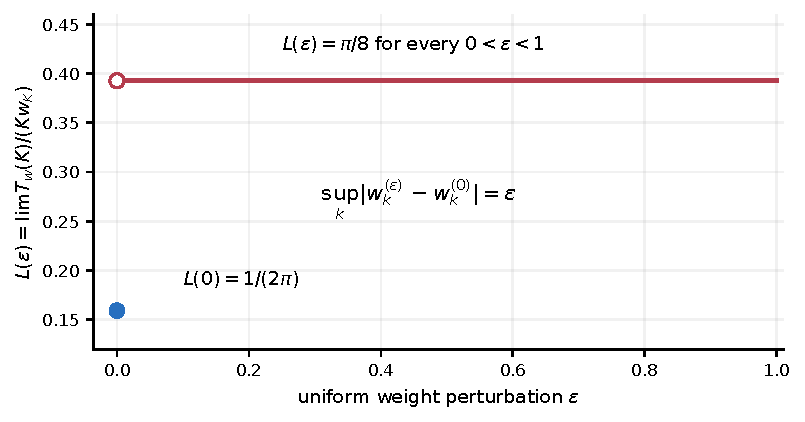
\includegraphics[width=.87\linewidth]{figures/03-schedules-constant_discontinuity.pdf}
 \caption{The proved discontinuity in the leading normalized threshold
 constant for \eqref{rex:sch:eq:epsilon-weights}. The open endpoint on the upper
 branch excludes $\varepsilon=0$; its filled value lies on the lower
 branch. This is a plot of the exact formulas, not an extrapolation of
 finite-horizon data.}
 \label{rex:sch:fig:jump}
\end{figure}

\subsection{Perturbations smaller than every inverse power}

\begin{theorem}[Identical algebraic expansions, different constants]
\label{rex:sch:thm:flat-perturbation}
Let $A\subseteq\N$ have natural density $\theta\in[0,1]$, and let
$0<h_j<1$ with $h_j\to0$. Define
\begin{equation}\label{rex:sch:eq:density-weights}
 w_{2j-1}=j,\qquad w_{2j}=j+h_j\ind_A(j).
\end{equation}
Then $w_k\sim k/2$ and
\begin{equation}\label{rex:sch:eq:density-L}
 \boxed{\displaystyle
 L_\theta=\frac12
 \left[\frac{\Gamma(1+\theta/2)}
 {\Gamma((1+\theta)/2)}\right]^2,\qquad
 \tau_w(n)\sim
 2\frac{\Gamma((1+\theta)/2)}{\Gamma(1+\theta/2)}\sqrt n.}
\end{equation}
In particular, choose $h_j=\varepsilon2^{-j^2}$ with $0<\varepsilon<1$.
Every schedule in this family satisfies
\begin{equation}\label{rex:sch:eq:flatness}
 w_k-\ceil{k/2}=o(k^{-N})\quad\text{for every }N>0,
\end{equation}
while its constant ranges continuously and strictly increasingly over
$[1/(2\pi),\pi/8]$ as $\theta$ ranges over $[0,1]$.
\end{theorem}

\begin{proof}
At even stages,
$\beta_{2j}=2h_j\ind_A(j)\to0$, and activity is exactly
$\ind_A(j)$. At odd stages,
\[
 \beta_{2j+1}
 =(2j+1)\frac{1-h_j\ind_A(j)}{j+h_j\ind_A(j)}\longrightarrow2.
\]
The joint empirical law is therefore
\[
 \mu_\theta=\tfrac12\delta_{(2,1)}
 +\tfrac\theta2\delta_{(0,1)}
 +\tfrac{1-\theta}{2}\delta_{(0,0)}.
\]
Its drift is $D_\theta(z)=(C(2z)+\theta)/2$.
Apply \cref{rex:sch:cor:one-positive} with $r=2,m=1,a=\theta$, and then
invert with $w_K\sim K/2$. The flatness assertion follows directly
from the chosen $h_j$. Strict monotonicity follows from the next
proposition, and continuity follows either from the Gamma formula
or from \cref{rex:sch:thm:continuity} below.
\end{proof}

An explicit set of every desired density is
\begin{equation}\label{rex:sch:eq:density-set}
 A_\theta=\{j\geq1:
 \lfloor(j+1)\theta\rfloor-\lfloor j\theta\rfloor=1\}.
\end{equation}
The count telescopes to $\theta N+O(1)$. Thus the family requires no
nonconstructive choice of a set of density $\theta$.

Equation \eqref{rex:sch:eq:flatness} gives a stronger obstruction than failure
of ordinary regular-variation universality. Even knowing the full
algebraic asymptotic expansions of the weights along both parity
classes leaves the leading extinction constant undetermined. The
missing datum is the occurrence of strictly positive perturbations
at the repeated weights.

\begin{proposition}[Quantitative dependence on activation]
\label{rex:sch:prop:activation}
Keep the positive-slope part of the drift fixed and write
$D_\eta=D_0+\eta$, where $D_0(0)>0$ and the available dormant mass
permits the stated values of $\eta$. Then
\begin{align}
 \log\frac{L(\eta_1)}{L(\eta_0)}
 &=(m+1)\int_0^\infty
 \frac{\eta_1-\eta_0}
 {(z+D_0(z)+\eta_0)(z+D_0(z)+\eta_1)}\dd z,
 \label{rex:sch:eq:activation-ratio}\\
 \frac{\dd}{\dd\eta}\log L(\eta)
 &=(m+1)\int_0^\infty\frac{\dd z}{(z+D_0(z)+\eta)^2}>0,
 \label{rex:sch:eq:activation-derivative}\\
 \frac{\dd^2}{\dd\eta^2}\log L(\eta)
 &=-2(m+1)\int_0^\infty\frac{\dd z}{(z+D_0(z)+\eta)^3}<0.
 \label{rex:sch:eq:activation-concavity}
\end{align}
Thus activation strictly increases $L$, with strictly concave
logarithm.
\end{proposition}

\begin{proof}
Use $\log L=\lim_{R\to\infty}[\log R-(m+1)H(R)]$ for the two
drifts and subtract. The difference integrand is integrable: the
denominator is bounded away from zero near the origin and grows
quadratically at infinity. This gives \eqref{rex:sch:eq:activation-ratio}.
The same bounds, locally uniform in $\eta$, permit differentiation
under the integral and prove the last two formulas.
\end{proof}

\begin{figure}[tbp]
 \centering
 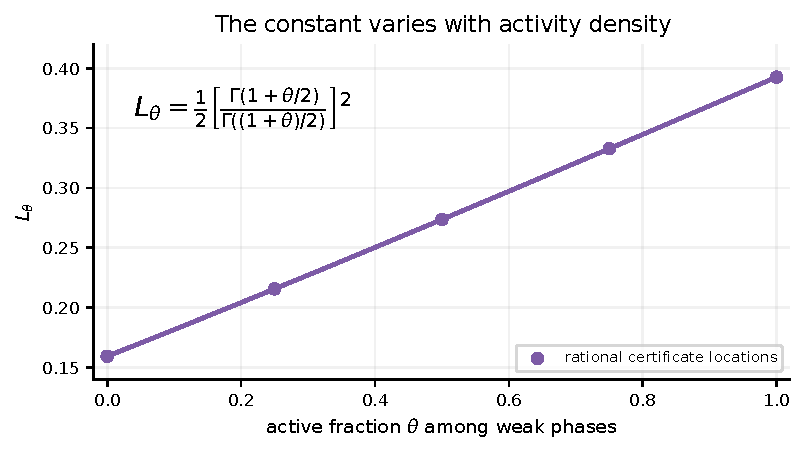
\includegraphics[width=.88\linewidth]{figures/03-schedules-weak_phase_density.pdf}
 \caption{The exact Gamma family \eqref{rex:sch:eq:density-L}. The marked
 density values are also covered by finite rational certificates in
 the accompanying data. The curve comes from the theorem; the
 displayed numerical evaluations are rounded.}
 \label{rex:sch:fig:density}
\end{figure}

\section{Periodic limiting slopes without a limiting constant}
\label{rex:sch:sec:no-limit}

The activity variable is necessary for existence as well as for the
value of a limit. We now remove the density assumption in
\cref{rex:sch:thm:flat-perturbation} in a controlled way.

\begin{theorem}[A fixed schedule with two subsequential constants]
\label{rex:sch:thm:no-limit}
There is a nondecreasing weight schedule with $w_k\sim k/2$,
$\beta_{2j}\to0$, and $\beta_{2j+1}\to2$, for which
$T_w(K)/(K w_K)$ does not converge. Two of its subsequential limits
are $1/(2\pi)$ and $\pi/8$.
\end{theorem}

\begin{proof}
Let $N_h=2^{2^h}$, for integers $h\geq1$. Define a set $A$ that is
alternately empty and full on the integer blocks
$[N_h,N_{h+1})$; its values before $N_1$ are arbitrary. Use
\eqref{rex:sch:eq:density-weights} with $h_j=1/(2j)$, and take horizons
\[
 K_h=2(N_{h+1}-1).
\]
The weights and slopes have the stated asymptotics regardless of
$A$, by the direct calculations in the previous proof.

Fix $\delta>0$. Since $N_h/N_{h+1}\to0$, all pairs whose stages
lie in $[\delta K_h,K_h]$ eventually belong to the last block,
apart from at most a bounded number of endpoints. Along the
subsequence of empty blocks, the joint empirical law on every
macroscopic time interval is the plateau law
$\mu_0=\frac12\delta_{(2,1)}+\frac12\delta_{(0,0)}$.
Along full blocks, it is the active-zero law
$\mu_1=\frac12\delta_{(2,1)}+\frac12\delta_{(0,1)}$.

The compactness and integrated-ceiling proof in
\cref{rex:sch:sec:proof-profile} uses only empirical averages within such
macroscopic intervals. It therefore applies along each of these
two horizon subsequences. Weight regular variation is already
available directly from $w_k\sim k/2$. The initial-tail estimate
\eqref{rex:sch:eq:tail-accounting} has, on either subsequence, normalized
upper limit $\delta^2/2$. Sending $\delta\downarrow0$ exactly as
in the threshold matching proof yields
\[
 \frac{T_w(K_h)}{K_hw_{K_h}}\longrightarrow
 \begin{cases}
 1/(2\pi),&\text{along empty terminal blocks},\\
 \pi/8,&\text{along full terminal blocks}.
 \end{cases}
\]
The constants differ. Earlier blocks disappear from the fixed
macroscopic interval and are controlled by the separate tail bound;
they have not been silently replaced by a global density assumption.
\end{proof}

The same proof works with $h_j=\varepsilon2^{-j^2}$. Thus even
weights agreeing with the repeated schedule to every algebraic
order can lack a normalized threshold limit.

\section{Where the lost mass goes}
\label{rex:sch:sec:losses}

The average residual $E(z)=D(z)-mz$ already gives
\begin{equation}\label{rex:sch:eq:ordinary-loss-density}
 -F'(t)=\frac{t^m}{L}E(z(t))\quad\text{a.e. on }(0,1).
\end{equation}
It describes the limiting distribution of the time at which an
infinitesimal fraction of the initial mass is removed. Keeping the
local increment state reveals which kinds of steps cause that loss.

\begin{theorem}[Joint loss time and increment state]\label{rex:sch:thm:loss}
Under \cref{rex:sch:thm:main}, let $J=\tau_w(n)$. The probability measures
\begin{equation}\label{rex:sch:eq:loss-measure}
 \nu_n=\sum_{k=2}^J\frac{x_{k-1}-x_k}{n}
 \delta_{(k/J,\beta_k,\sigma_k)}
\end{equation}
converge weakly on $[0,1]\times\mathcal E_B$ to
\begin{equation}\label{rex:sch:eq:marked-loss-limit}
 \boxed{\displaystyle
 \frac{t^m}{L}
 \bigl(\sigma C(\beta z(t))-\beta z(t)\bigr)
 \dd t\,\mu(\dd\beta,\dd\sigma).}
\end{equation}
The limiting loss mass carried by state $(0,1)$ equals
\begin{equation}\label{rex:sch:eq:weak-loss-fraction}
 \frac{\eta}{(m+1)L}.
\end{equation}
\end{theorem}

\begin{proof}
On a compact interval $[\delta,1-\delta]$, the positive forward
quotients satisfy $Q_k/J\to y(k/J)$ uniformly. The integer
$d'_k=Q_{k-1}-Q_k$ obeys, directly from the floor recurrence,
\begin{equation}\label{rex:sch:eq:forward-decrement}
 b_kQ_k\leq d'_k<b_kQ_k+1+b_k.
\end{equation}
When $b_k=0$, this forces $d'_k=0$. When $b_k>0$ and $b_kQ_k$
tends to zero, it forces $d'_k=1$ for sufficiently large $J$.
Away from small neighborhoods of positive integers in
$\beta_k z(k/J)$, the only integer allowed by
\eqref{rex:sch:eq:forward-decrement} is
$\sigma_k C(\beta_k z(k/J))$. The joint averaging argument of
\cref{rex:sch:lem:joint} shows that the exceptional neighborhoods have
vanishing limiting empirical mass as their widths tend to zero.
All terms are uniformly bounded on the chosen compact interval.

The exact loss at a step is
\[
 x_{k-1}-x_k=w_{k-1}
 \left(d'_k-\beta_k\frac{Q_k}{k}\right).
\]
Use $w_{k-1}/w_J\to(k/J)^m$ and $n/(Jw_J)\to L$, then apply
joint averaging against any continuous test function. This gives
\eqref{rex:sch:eq:marked-loss-limit} on the compact time interval.
The total omitted early loss has limiting upper bound
$1-F(\delta)$, and the late loss has upper bound $F(1-\delta)$,
by uniform forward convergence. Both tend to zero when
$\delta\downarrow0$. Hence the full weak convergence follows.

The density is nonnegative and its total integral is one by
\eqref{rex:sch:eq:mass-integral}. At state $(0,1)$ its residual factor is
exactly one; integrating $\eta t^m/L$ over time proves
\eqref{rex:sch:eq:weak-loss-fraction}.
\end{proof}

For a general empirical law, \eqref{rex:sch:eq:weak-loss-fraction} refers
to the atom in the \emph{limiting} measure. It can be measured by
first including active states with $0<\beta_k\leq a$, taking the
large-$n$ limit at continuity values of $a$, and then sending
$a\downarrow0$. It does not assert that a finite-stage pair can
equal $(0,1)$. In finite-type examples with a separated positive
slope, it is simply the fraction lost at the designated
zero-slope active phases.

For \eqref{rex:sch:eq:epsilon-weights} with $\varepsilon>0$,
$\eta=1/2$, $m=1$, and $L=\pi/8$. Therefore the even steps remove
an asymptotic fraction
\begin{equation}\label{rex:sch:eq:two-over-pi-loss}
 \frac{2}{\pi}=0.6366197723\ldots
\end{equation}
of the initial mass. Their increments in the weights tend to zero,
yet their rounding losses remain a macroscopic portion of the total.
At the relevant stages the input is close to a multiple of the
previous weight; increasing that weight by any positive amount
can force the integer quotient down by one. The theorem makes
that mechanism quantitative without a random-fractional-part model.

The product measure used in \cref{rex:sch:lem:joint} describes one stage
sampled at a macroscopic time. It does not say that consecutive
phases of a periodic or deterministic schedule are independent.

\section{Continuity and bounded sparse exceptions}
\label{rex:sch:sec:stability}

The instability above has a complementary positive result. The
constant is continuous when the activity information is retained.

\begin{theorem}[Continuity in the augmented increment law]
\label{rex:sch:thm:continuity}
Let $\mu_j\weak\mu$ on a common compact state space $\mathcal E_B$,
with $m=\int\beta\dd\mu>0$. Write $m_j,D_j,H_j,L_j,F_j$ for
the corresponding quantities, restricting to the sufficiently large
$j$ for which $m_j>0$. Then
\[
 m_j\to m,\qquad L_j\to L,
 \qquad \sup_{0\leq t\leq1}|F_j(t)-F(t)|\to0.
\]
The backward profiles converge locally uniformly on $(0,1]$.
\end{theorem}

\begin{proof}
The mean and activity are continuous functions of the law, so
$m_j\to m>0$ and $\rho_j\to\rho>0$. For all but countably many
$z>0$, the bounded function $(\beta,\sigma)\mapsto\sigma C(\beta z)$
is $\mu$-almost everywhere continuous. The exceptional $z$ occur
when a positive atom $\beta$ of $\mu$ satisfies $\beta z\in\N$.
Thus $D_j(z)\to D(z)$ for almost every $z$.
Since $D_j(z)\geq\rho_j$, dominated convergence on bounded
$z$-intervals yields locally uniform convergence $H_j\to H$.
Strict monotonicity and continuity of the integrals give convergence
of their inverses, and hence of $y_j$, on compact time intervals.

To pass from a fixed $R$ to $L_j$, use the weaker form of
\eqref{rex:sch:eq:certificate} with lower endpoint
$R e^{-(m_j+1)H_j(R)}$ and upper-to-lower ratio at most
$1+1/((m_j+1)R)$. The lower endpoint converges for fixed $R$.
Let $R\to\infty$ after $j\to\infty$; this proves $L_j\to L$.
Local convergence of $F_j$ follows. Finally,
\[
 0\leq1-F_j(t)\leq
 \frac{\rho_j}{(m_j+1)L_j}t^{m_j+1},
\]
which controls the initial endpoint uniformly. Continuity and
monotonicity of the profiles control the terminal endpoint.
\end{proof}

In particular, a positive slope tending to zero approaches the
state $(0,1)$. Its limiting drift contribution is one times its
frequency. Assigning that limit to $(0,0)$ changes the law, which
explains the discontinuity of the unaugmented description.

\begin{corollary}[Bounded changes on a density-zero set]
\label{rex:sch:cor:sparse}
Suppose two nondecreasing schedules have bounded scaled increments
and agree in their successive ratios outside a set
$E\subseteq\N$ with $\#(E\cap[1,N])=o(N)$. If the first
augmented empirical law converges with positive mean, then the
second has the same limiting law. Their constants $L$, backward
profiles, and normalized forward profiles coincide.
\end{corollary}

\begin{proof}
For a bounded continuous test function, the two empirical averages
differ in absolute value by at most twice its supremum norm times
$\#(E\cap[1,N])/(N-1)$, which tends to zero. Apply
\cref{rex:sch:thm:main} to both schedules.
\end{proof}

The normalization in this conclusion uses each schedule's own
$w_K$. Sparse changes in ratios can accumulate into a nontrivial
factor in the weights themselves. Thus the corollary asserts
$T_w(K)/(K w_K)\to L$ and
$T_{\widetilde w}(K)/(K\widetilde w_K)\to L$; it does not
assert $T_{\widetilde w}(K)/T_w(K)\to1$ without a corresponding
comparison of the weights. Unbounded exceptional increments are
outside the corollary's assumptions.

[Added 7 October 2026, batch~110: this answers the bounded form of Part~I's
Research question~\ref{rex:q:sparse}. If nondecreasing weights satisfy
$k(w_k/w_{k-1}-1)\to m$ outside a set of density zero and their scaled
increments are bounded on that set, they agree in their successive ratios,
off that set, with nondecreasing weights whose ratios satisfy the
hypothesis everywhere (put $w_k/w_{k-1}=1+m/k$ on the exceptional set), so
their augmented law is $\delta_{(m,1)}$ and their constant is $L_m$. Part~I's
question whether a sparse set of very large jumps can change the constant
is Research question~\ref{rex:sch:q:sparse} below, open.]

\section{The sharp spectrum and equivalence of normalized shapes}
\label{rex:sch:sec:spectrum}

The previous examples vary a constant while preserving the mean
slope. The full possible range can also be determined.

\begin{proposition}[Activity bound and scaling]\label{rex:sch:prop:scaling}
Every law in \cref{rex:sch:thm:main} satisfies
\begin{equation}\label{rex:sch:eq:activity-lower}
 L\geq\frac{\rho m^m}{(m+1)^{m+1}}.
\end{equation}
For a finite-type drift $D$ and any $0<c\leq1$, multiply every
active frequency by $c$, every positive slope by $1/c$, and put
the remaining mass in a dormant type. The resulting drift and
constant satisfy
\begin{equation}\label{rex:sch:eq:thinning}
 D_c(z)=cD(z/c),\qquad
 t_c(z)=t(z/c),\qquad y_c(t)=cy(t),\qquad L_c=cL.
\end{equation}
The mean slope and normalized forward shape remain unchanged.
\end{proposition}

\begin{proof}
The terminal selection inequality gives
$y(t)\geq\rho(1-t)$. Since $L\geq t^my(t)$, maximize
$\rho t^m(1-t)$ at $t=m/(m+1)$ to obtain
\eqref{rex:sch:eq:activity-lower}. The drift identity in
\eqref{rex:sch:eq:thinning} follows directly from the phase construction,
including its active zero types. In the integral defining $H_c$,
substitute $u=cv$ to get $H_c(z)=H(z/c)$. The remaining
identities and invariance of $F=t^my/L$ follow.
\end{proof}

\begin{theorem}[Every interior constant is attainable]
\label{rex:sch:thm:spectrum}
Fix $m>0$. Among the nondecreasing positive real weight schedules
with a convergent bounded augmented increment law of mean $m$,
the set of normalized constants is exactly
\begin{equation}\label{rex:sch:eq:spectrum}
 \boxed{\displaystyle \{L\}=\left(0,\frac1{m+1}\right).}
\end{equation}
Every value can be realized by a finite-type schedule. It can
also be realized with the additional normalization $w_K\sim K^m$,
so that $T_w(K)\sim L K^{m+1}$.
The finite bound on the increments may depend on the desired
constant; a single bound prescribed for all schedules is not assumed.
\end{theorem}

\begin{proof}
The strict inclusion in the displayed interval is already proved
in \eqref{rex:sch:eq:universal-bounds}. To approach its upper endpoint,
take the finite law with positive slope $rm$ of frequency $1/r$
and active-zero mass $1-1/r$, for an integer $r\geq1$. Its drift is
\[
 D_r(z)=1-\frac1r+\frac1r C(rmz),
\]
and its residual lies between $1-1/r$ and $1$. Therefore
\begin{equation}\label{rex:sch:eq:upper-approach}
 \frac{1-1/r}{m+1}\leq L_r<\frac1{m+1},
 \qquad L_r\longrightarrow\frac1{m+1}.
\end{equation}
Given any $0<\ell<1/(m+1)$, choose $r$ with $L_r>\ell$ and
set $c=\ell/L_r$. Apply \cref{rex:sch:prop:scaling}. The new finite law
has mean $m$ and constant $cL_r=\ell$.

It remains to realize possibly irrational frequencies by actual
weights with a controlled leading asymptotic. For a finite
alphabet with frequencies $p_s$, let block $h$ have length $h$.
Assign each active symbol $s$ exactly $\lfloor p_sh\rfloor$
positions in that block, and assign the remainder to the dormant
symbol. Arrange the block in any fixed order. The counts satisfy
\begin{equation}\label{rex:sch:eq:discrepancy}
 N_s(N)=p_sN+O(\sqrt N).
\end{equation}
Indeed, the cumulative rounding error through block $h$ is $O(h)$,
and an incomplete final block has length $O(h)$, while the total
length is $h(h+1)/2$.

At position $k\geq2$, choose the ratio
\begin{equation}\label{rex:sch:eq:realization-ratios}
 \frac{w_k}{w_{k-1}}=
 \begin{cases}
 1+\alpha_s/k,&\text{a positive-slope type }s,\\
 1+k^{-2},&\text{an active zero-slope type},\\
 1,&\text{a dormant type},
 \end{cases}
 \qquad w_1=1.
\end{equation}
This realizes the required augmented law. Set $a_k=\alpha_s$
on positive types and $a_k=0$ otherwise. By
\eqref{rex:sch:eq:discrepancy},
$\sum_{k\leq N}(a_k-m)=O(\sqrt N)$. Abel summation shows that
$\sum_{k\leq N}(a_k-m)/k$ converges, with error $O(N^{-1/2})$.
Also $\log(w_k/w_{k-1})=a_k/k+O(k^{-2})$. Hence
\begin{equation}\label{rex:sch:eq:realization-weight}
 w_N=A N^m\bigl(1+O(N^{-1/2})\bigr)
\end{equation}
for some $A>0$.

To obtain $w_N\sim N^m$, choose $N_0$ so large that
$A^{-1}w_{N_0}\geq1$. Set the first $N_0-1$ weights equal to
one and replace the tail by $A^{-1}w_k$ for $k\geq N_0$.
The new sequence is nondecreasing, starts at one, and has the same
successive ratios after one transition. Its augmented law and
constant are unchanged. The one exceptional finite ratio has a
finite scaled increment, so the boundedness hypothesis remains
valid after increasing its bound.
\end{proof}

This theorem concerns positive real weights, as does the real-power
version of the original OEIS question. It does not assert the same
spectrum under an additional requirement that every weight be an
integer. The construction also uses dormant phases; it is not a
claim about the smaller class in which every transition must be
strictly increasing.

The approximating constants have an explicit form, useful for
constructing the desired law:
\begin{equation}\label{rex:sch:eq:Lr-gamma}
 L_r=\frac1{rm}
 \left[
 \frac{\Gamma((rm+1)/(m+1))}
 {\Gamma(rm/(m+1))}
 \right]^{m+1}
 =\frac1{m+1}\left(1-\frac1{2r}+O_m(r^{-2})\right).
\end{equation}
The exact identity is \cref{rex:sch:cor:one-positive} with $a=r-1$.
The expansion follows from the first correction in the standard
Gamma-ratio expansion \cite[\S5.11(iii)]{dlmf}. The bounds
\eqref{rex:sch:eq:upper-approach} alone suffice for the spectrum proof.

\begin{proposition}[When two normalized trajectories agree]
\label{rex:sch:prop:shape}
Consider two laws with the same mean $m>0$. Their normalized
forward profiles agree if and only if
\begin{equation}\label{rex:sch:eq:shape-classification}
 D_2(z)=cD_1(z/c)\quad\text{for almost every }z>0,
 \qquad c=L_2/L_1.
\end{equation}
\end{proposition}

\begin{proof}
The drift relation gives the integral change of variables used in
\cref{rex:sch:prop:scaling}, so it implies equality of the normalized
profiles. Conversely, equality of $F_1$ and $F_2$ gives
$y_2=cy_1$. Differentiating their locally absolutely continuous
representatives and using the differential equation yields
\[
 D_2(cz_1(t))=cD_1(z_1(t))\quad\text{for a.e. }t.
\]
The map $t\mapsto z_1(t)$ and its inverse are locally Lipschitz
away from the endpoints, by \eqref{rex:sch:eq:z-ode} and the local drift
bounds. They preserve null sets locally, so the identity transfers
to almost every $z>0$. The integral formulas are insensitive to changes
at individual jump points. With the fixed ceiling convention used here,
those values are determined by left continuity.
\end{proof}

\begin{theorem}[Exact recovery of every bounded law]
\label{rex:sch:thm:recovery}
The drift $D$ determines the entire augmented increment law $\mu$
on $\mathcal E_B$. In particular, let $\mathfrak m(n)$ be the
arithmetic M\"obius function, characterized by
$\sum_{d\mid n}\mathfrak m(d)=\ind_{\{n=1\}}$, and put
$f(x)=\mu\{(\beta,\sigma):\beta>x\}$ for $x>0$. Then
\begin{equation}\label{rex:sch:eq:mobius-recovery}
 \boxed{\displaystyle
 f(x)=\sum_{1\leq n\leq B/x}\mathfrak m(n)
 \left[D\!\left(\frac1{nx}\right)-\rho\right],
 \qquad \rho=\lim_{z\downarrow0}D(z).}
\end{equation}
Every sum is finite. The remaining masses are
\begin{equation}\label{rex:sch:eq:recover-zero}
 \mu\{(0,1)\}=\rho-\lim_{x\downarrow0}f(x),
 \qquad \mu\{(0,0)\}=1-\rho.
\end{equation}
Knowing $D$ almost everywhere suffices, since its canonical
representative is left-continuous on $(0,\infty)$.
\end{theorem}

\begin{proof}
For $u\geq0$, the chosen convention gives the exact identity
\[
 C(u)=1+\sum_{j\geq1}\ind_{\{u>j\}}.
\]
All positive slopes have activity flag one. Integrating and
substituting $z=1/x$ therefore gives
\[
 G(x):=D(1/x)-\rho=\sum_{j\geq1}f(jx).
\]
Because the slopes are bounded by $B$, terms with $jx\geq B$
vanish. The proposed inverse can consequently be rearranged as
a finite sum:
\[
 \sum_{n\geq1}\mathfrak m(n)G(nx)
 =\sum_{n,j\geq1}\mathfrak m(n)f(jnx)
 =\sum_{k\geq1}f(kx)\sum_{n\mid k}\mathfrak m(n)
 =f(x).
\]
This proves \eqref{rex:sch:eq:mobius-recovery}. The tail function $f$
determines the positive-slope measure, including all its atoms.
Its total mass is $\lim_{x\downarrow0}f(x)$. The activity
and total masses then give \eqref{rex:sch:eq:recover-zero}.

For each fixed $\beta>0$, $C(\beta z)$ is left-continuous in
$z>0$, and for $\beta=0$ it is constant. Bounded convergence
on compact $z$-intervals proves left continuity of $D$.
Two left-continuous functions agreeing almost everywhere agree
everywhere on $(0,\infty)$, which proves the final assertion.
\end{proof}

Thus an exact backward profile determines the law: its differential
equation gives $D(z(t))=-y'(t)$ almost everywhere, and the coordinate
change used in \cref{rex:sch:prop:shape} transfers that information to
$z$-space. The schedule's ordering is absent from the law and is
not recoverable. If only the normalized forward shape is known
at a fixed $m$, \cref{rex:sch:prop:shape} describes the remaining scaling
ambiguity. Formula~\eqref{rex:sch:eq:mobius-recovery} addresses exact data;
it is not an assertion of stable recovery from noisy observations.

\section{Exact computations and numerical illustrations}
\label{rex:sch:sec:computations}

The accompanying program checks the discrete definitions separately
from the asymptotic calculations. It uses integer ceiling and floor
division for all threshold and survival decisions. The integer
recurrence is short enough to describe completely.

\subsection{Exact algorithms and conventions}

If a successive ratio is the positive rational $a_k/b_k$, the
backward update is
\begin{equation}\label{rex:sch:eq:algorithm}
 q\ \longleftarrow\
 \left\lfloor\frac{a_kq+b_k-1}{b_k}\right\rfloor.
\end{equation}
The forward quotient update is
$Q\leftarrow\lfloor b_kQ/a_k\rfloor$. Both are exact integer
operations. A single threshold calculation uses $K-1$ updates;
this operation count does not treat arbitrary-size integer
arithmetic as unit cost.

For a periodic tuple $(\alpha_0,\ldots,\alpha_{p-1})$, the
implemented transition $k-1\to k$ uses $\alpha_{k\bmod p}$,
for $k\geq2$. Positive phases use ratio $1+\alpha_{k\bmod p}/k$;
an active zero phase uses $1+k^{-2}$; a dormant phase uses one.
Thus the tuple $(1)$ in the numerical tables has
$w_k=(k+1)/2$, not $w_k=k$. It has the same limiting drift and
$L=1/\pi$, but its finite thresholds differ from A002491.
No newly computed table is presented as an existing OEIS b-file.

For \eqref{rex:sch:eq:epsilon-weights}, if $\varepsilon=a/b$ in lowest
terms, the exact ratios are
\begin{equation}\label{rex:sch:eq:epsilon-rational-ratios}
 r_{2j}=\frac{bj^2+a}{bj^2},\qquad
 r_{2j+1}=\frac{bj(j+1)}{bj^2+a}.
\end{equation}
The weights at the selected horizons are available directly, so
no numerical product is needed to define that model.

\subsection{Recorded verification scope}

The completed run records the following results in
\texttt{data/verification.json}:
\begin{itemize}
 \item 3,200 exact boundary checks across ten models, for every
 horizon $K\leq40$ and terminal target quotient $1,2,3,4$.
 The computed backward threshold reaches the terminal target;
 decreasing the initial integer by one does not.
 \item 2,847 exhaustive small-survival comparisons at $K\leq15$,
 covering initial integers through slightly above each threshold.
 \item 310 exact integer thresholds, including the horizons
 $100,1000,10000,100000$.
 \item 22 finite rational certificates, including five activation
 densities and endpoints $z=100$ and $z=1000$.
\end{itemize}
All recorded checks passed. They verify implementations and finite
identities on their stated ranges; they are not a substitute for
the asymptotic proofs.

\begin{table}[tbp]
 \centering\small
 \begin{tabular}{@{}rrrr@{}}
 \toprule
 $\varepsilon$ & $T_w(100000)$ & $T_w(K)/(K w_K)$ & Predicted $L$\\
 \midrule
 $0$ & $795767254$ & $0.159153450800$ & $0.159154943092$\\
 $1/2$ & $1962394026$ & $0.392478805122$ & $0.392699081699$\\
 $1/100$ & $1963448713$ & $0.392689742598$ & $0.392699081699$\\
 $1/10000$ & $1963518231$ & $0.392703646200$ & $0.392699081699$\\
 \bottomrule
 \end{tabular}
 \caption{Exact thresholds for \eqref{rex:sch:eq:epsilon-weights} at
 $K=100000$. Decimal ratios and constants are rounded numerical
 displays. The convergence for $\varepsilon=1/2$ is visibly slower
 than for the smaller perturbations; a rate is not inferred.}
 \label{rex:sch:tab:epsilon}
\end{table}

\begin{table}[tbp]
 \centering\small
 \begin{tabular}{@{}lrrr@{}}
 \toprule
 Positive slope tuple & $T_w(100000)$ & Normalized value & Predicted $L$\\
 \midrule
 $(1)$ & $1591627536$ & $0.318322323977$ & $0.318309886184$\\
 $(1/2,3/2)$ & $1432132519$ & $0.331907175562$ & $0.331897673629$\\
 $(1/2,1,3/2)$ & $1708313875$ & $0.329295202144$ & $0.329276508811$\\
 $(1/2,3/2,1)$ & $1520900013$ & $0.329280395971$ & $0.329276508811$\\
 \bottomrule
 \end{tabular}
 \caption{Positive periodic phases. The last two rows have the
 same empirical law and therefore the same normalized limit,
 despite their different finite weights and thresholds. All
 displayed decimals are rounded.}
 \label{rex:sch:tab:positive}
\end{table}

\begin{figure}[tbp]
 \centering
 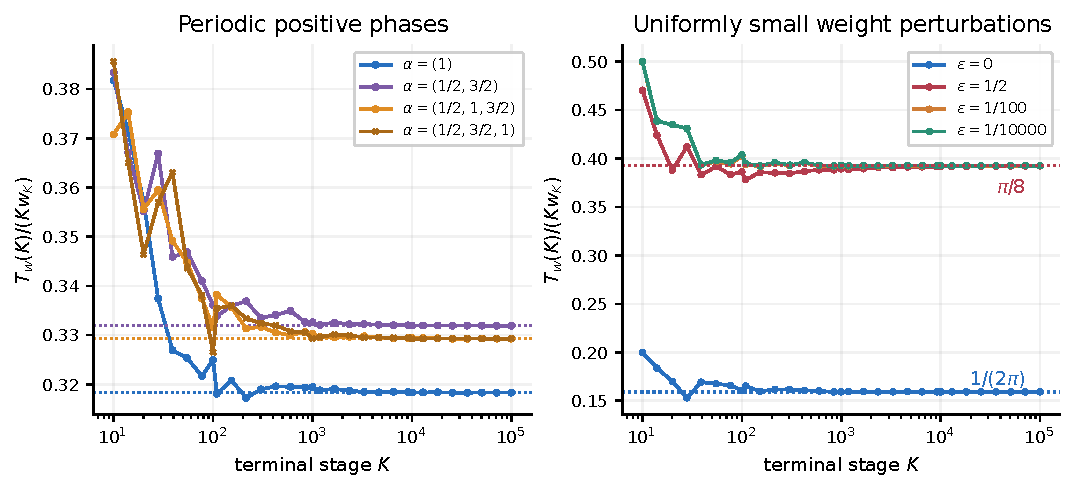
\includegraphics[width=\linewidth]{figures/03-schedules-normalized_thresholds.pdf}
 \caption{Exact thresholds divided by numerical evaluations of
 $K w_K$. Horizontal reference values are proved constants.
 The finite-horizon curves are diagnostics of convergence,
 with no fitted error law asserted.}
 \label{rex:sch:fig:thresholds}
\end{figure}

\begin{figure}[tbp]
 \centering
 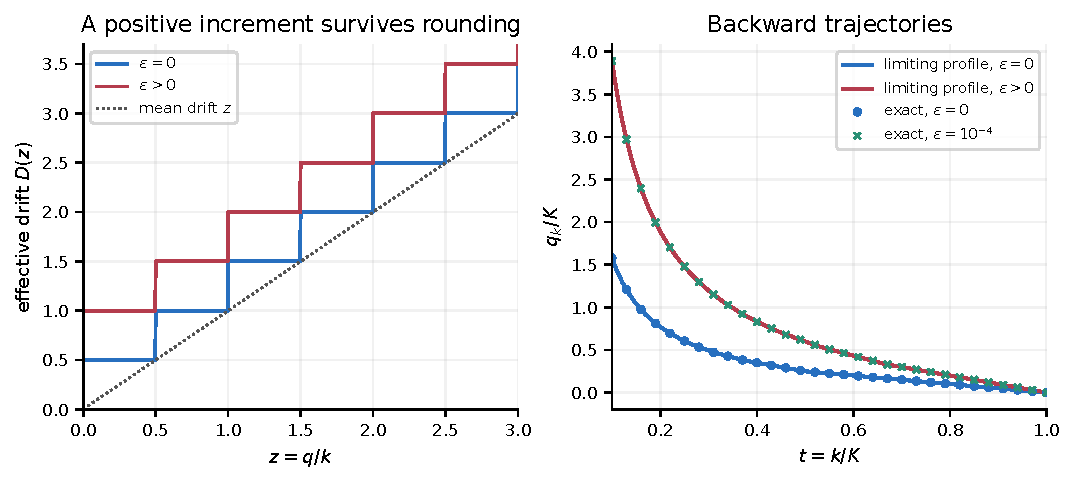
\includegraphics[width=\linewidth]{figures/03-schedules-drift_and_profiles.pdf}
 \caption{The ceiling drift and backward quotient profiles for
 the repeated-weight and active-zero examples. Markers use exact
 integer quotient arrays; smooth segments represent the explicit
 limiting solution. The difference between the limiting curves
 persists as the perturbation size tends to zero through positive
 values.}
 \label{rex:sch:fig:profiles}
\end{figure}

\subsection{Certificates versus rounded numerical values}

The certificate file stores the numerator and denominator of each
endpoint in \eqref{rex:sch:eq:certificate}, evaluated through the finite
product \eqref{rex:sch:eq:finite-product}. These fractions are exact.
The printed decimal approximations in \cref{rex:sch:tab:certificates}
are rounded displays of those endpoints, not claims of directed
decimal rounding. In particular, inequalities should be checked
against the stored fractions when every digit matters.

\begin{table}[tbp]
 \centering\small
 \begin{tabular}{@{}lrr@{}}
 \toprule
 Drift & Lower endpoint & Upper endpoint\\
 \midrule
 $C(z)$ & $0.318230318662$ & $0.318389433821$\\
 $\tfrac12C(z/2)+\tfrac12C(3z/2)$
 & $0.331814703827$ & $0.331980611179$\\
 $\tfrac12C(2z)$ & $0.159135049968$ & $0.159174833730$\\
 $\tfrac12(C(2z)+1)$ & $0.392650009649$ & $0.392748147617$\\
 \bottomrule
 \end{tabular}
 \caption{Rounded displays of exact rational finite-product
 certificate endpoints at $z=1000$. These enclose the limiting
 constants, not the finite-$K$ threshold ratios.}
 \label{rex:sch:tab:certificates}
\end{table}

For the periodic weight products, the program uses 70-digit
\texttt{Decimal} arithmetic. General Gamma-product displays use
ordinary floating-point log-Gamma evaluations. Those evaluations
are explicitly labeled as numerical diagnostics. The exact
threshold recurrences and the exact rational certificate fractions
do not depend on those floating-point values.

\FloatBarrier
\subsection{Reproducing the package}

From the archive directory, run
\begin{quote}\ttfamily
python3 code/verify.py
\end{quote}
to recreate the data and figures. Add \texttt{-{}-no-figures} to
run the arithmetic without NumPy or Matplotlib. The source and
arithmetic use Python's standard library; figure generation uses
NumPy and Matplotlib. Compile the paper with
\begin{quote}\ttfamily\small
latexmk -pdf -interaction=nonstopmode periodic\_rounding\_extinction.tex
\end{quote}
The archive includes the compiled PDF and every figure required by
the LaTeX source, so reproduction of the figures is optional.
The source audit and verification notes describe precisely which
results were checked and which remain open.

[Added 7 October 2026, batch~110: this section describes the delivered
archive. In this report the program is \path{code/03-schedules-verify.py},
its recorded outputs are \path{data/03-schedules-*} (the file named above as
\texttt{data/verification.json} is
\path{data/03-schedules-verification.json}), the figures are
\path{figures/03-schedules-*}, and the source audit and verification notes
are \path{03-schedules-SOURCE_AUDIT.txt} and
\path{03-schedules-VERIFICATION_NOTES.txt}. The delivered PDF, the
delivered \texttt{README.txt} and the checksum manifest are not shipped. The
program writes \texttt{data/} and \texttt{figures/} under the directory
given by \texttt{-{}-output}, by default the directory above its own, with
the delivered file names; run in place it would add unprefixed files to
this report, so the report's \texttt{README.md} runs it on a copy with an
explicit output directory.]

\section{Further research questions}
\label{rex:sch:sec:questions}

The following questions are proposed continuations of this article.
Except where an older conjecture is explicitly identified, their
open status is relative to the results proved here and the sources
examined, rather than a claim about every publication.

\begin{question}[Quantitative averaging and threshold errors]\label{rex:sch:q:quant}
For a fixed finite periodic schedule with
$\beta_k=\alpha_{k\bmod r}+O(k^{-1})$, obtain an explicit
error bound in $T_w(K)=LK w_K+E(K)$ and in the full trajectory.
How does the rate depend on the smallest positive slope and on
the presence of active zero phases?
\end{question}

A proof must track the accumulated crossing errors and balance
them against the singular initial tail. The empirical theorem
provides no rate when the empirical law itself has no rate.
For \eqref{rex:sch:eq:epsilon-weights}, the heuristic balance
$\varepsilon q_k/k^2\asymp1$ with $q_k\asymp K^2/k$ suggests
a scale $k\asymp\varepsilon^{1/3}K^{2/3}$. This is only a guide
for a quantitative argument, not a proved boundary-layer estimate.

[Added 7 October 2026, batch~110: Part~II proves such a bound in the
one-type case of exact powers, $w_k=k^m$:
$T_m(K)=L_mK^{m+1}+O_m(K^{(m+1)^2/(m+2)})$, with an explicit enclosure
(\cref{rex:qt:thm:main,rex:qt:thm:envelope}). Its drift sandwich
(\cref{rex:qt:lem:drift}) uses the power grid, so even general weights with
the law $\delta_{(m,1)}$ are not covered, and every periodic schedule with
more than one type stays open.]

\begin{question}[The classical bounded-error conjecture]\label{rex:sch:q:classical}
Resolve $T_{k}(K)=K^2/\pi+O(K)$, equivalently
$\tau_k(n)=\sqrt{\pi n}+O(1)$, and determine the appropriate
counterparts for power or periodic schedules.
\end{question}

The proved classical error $O(K^{4/3})$ is the reliable benchmark
\cite{erdos-jabotinsky}. OEIS A002491 records Knuth's objection to the error
summation in the later claimed sharpening \cite{oeis-threshold}.
The present article does not settle that issue. A recent preprint
of Li studies the ordinary two-dimensional array with an
$O((i+j+1)^{4/3})$ estimate \cite{li}; it does not supply a
periodic-weight error theorem used here.

[Added 7 October 2026, batch~110: this is Part~I's Research
question~\ref{rex:q:bounded} and Part~II's question~\ref{rex:qt:q:bounded};
Part~II's remainder at $m=1$ is the classical $O(K^{4/3})$. Open.]

\begin{question}[A fixed slope bound and strict increase]\label{rex:sch:q:fixedB}
For prescribed $m$, $B$, and activity frequency $\rho$, determine
the attainable interval of $L$ under $0\leq\beta_k\leq B$.
What is the sharp range if every step is strictly increasing?
\end{question}

The spectrum theorem allows a different finite $B$ for each
construction, and its thinning argument introduces dormant steps.
The lower bound \eqref{rex:sch:eq:activity-lower} becomes relevant when
$\rho$ is fixed. Optimizing the ceiling average under a mean
constraint is a distinct problem from optimizing an affine drift.

\begin{question}[Integer weights]\label{rex:sch:q:integer}
Which constants can be realized when every $w_k$ is a positive
integer, with $w_k\sim A k^m$? Which real-weight constructions
survive a final rounding of the weights themselves?
\end{question}

The flat perturbation examples are deliberately real-valued.
Rounding their weights to integers can erase the activity datum
that causes the effect. Thus the integer restriction cannot be
added to \cref{rex:sch:thm:spectrum} without another proof.

\begin{question}[Unbounded and signed local increments]\label{rex:sch:q:unbounded}
Replace the uniform bound on $\beta_k$ by an integrability or
uniform-integrability condition, and determine whether a comparable
law holds when some scaled increments are negative but the mean
growth index is positive.
\end{question}

Rare large increments can be negligible in frequency and still
affect the weighted trajectory. Negative phases remove the
stepwise monotonicity used to prove transversality before
averaging. Both modifications require new estimates; the current
theorem does not cover them.

\begin{question}[Sparse large jumps]\label{rex:sch:q:sparse}
Find necessary or sufficient conditions on a density-zero
exceptional set and its total logarithmic weight change that
preserve the profile and constant when its scaled increments are
not uniformly bounded.
\end{question}

The bounded case is \cref{rex:sch:cor:sparse}. A successful extension
must control both the exceptional quotient jumps and their
contribution to the small-time weighted tail, rather than using
density alone.

[Added 7 October 2026, batch~110: this is the part of Part~I's Research
question~\ref{rex:q:sparse} that \cref{rex:sch:cor:sparse} leaves open.
Together with Research questions~\ref{rex:sch:q:unbounded}
and~\ref{rex:sch:q:nonconv}, it is also what remains of Part~I's Research
question~\ref{rex:q:schedules} outside the class of
\cref{rex:sch:thm:main}.]

\begin{question}[Quantitative recovery from approximate trajectories]\label{rex:sch:q:recovery}
Given noisy or finitely sampled observations of a backward profile,
how accurately can its bounded augmented increment law be recovered?
Under what separation or regularity assumptions are the positive
slopes, their frequencies, and the active-zero mass stably identifiable?
\end{question}

Theorem~\ref{rex:sch:thm:recovery} settles exact identification from $D$ for
every bounded law in the article, and \cref{rex:sch:prop:shape} identifies
the scaling ambiguity between normalized profiles. Quantitative
recovery is more delicate: obtaining $D$ from a profile requires
differentiation, and the M\"obius formula uses increasingly many terms
near zero slope. The scalar constant alone is insufficient; determining
optimal bounds on a law from that single statistic is another question.

\begin{question}[Nonconvergent environments]\label{rex:sch:q:nonconv}
For a schedule without a limiting augmented empirical law,
characterize the cluster set of $T_w(K)/(K w_K)$. How much of it
is determined by empirical laws on macroscopic time windows,
which may now depend on time?
\end{question}

The two-point construction in \cref{rex:sch:thm:no-limit} isolates two
homogeneous terminal environments. More general block schedules
can have multiple environmental regions on the same horizon,
suggesting a nonautonomous limiting equation whose coefficient
law depends on $t$.

\begin{question}[Random schedules and fluctuations]\label{rex:sch:q:random}
For bounded random local increments, derive fluctuations of the
threshold around its deterministic limit, under explicit mixing
or independence assumptions. Separate environmental fluctuations
from the arithmetic fluctuations caused by ceiling crossings.
\end{question}

The theorem is deterministic and applies to each realization with
the required empirical convergence. It provides a leading law but
does not establish a central limit theorem, a fluctuation scale,
or independence of successive phases.

\begin{question}[Symbolic constants beyond commensurable slopes]\label{rex:sch:q:symbolic}
For finitely many incommensurable positive slopes, study efficient
certified evaluation of $L$, arithmetic properties of its defining
product, and possible reductions to recognized special functions.
\end{question}

The integral and finite certificates remain valid, but there is no
common cell for \cref{rex:sch:thm:gamma}. The ordered union of distinct
crossing sets replaces the finite Gamma product. This is an
appropriate setting for symbolic and numerical investigation
without asserting an unsupported closed form.

\section{Proof dependencies and source audit}
\label{rex:sch:sec:audit}

The main logical chain is exact survival duality, weight-ratio
control, compactness with positive terminal drift, integrated
ceiling averaging, a unique separated differential equation, and
small-time matching. The constant enclosures follow from the
same differential equation, independently of finite-threshold
experiments. The Gamma formulas additionally use the Gamma
functional equation and its standard ratio asymptotic. The
instability and spectrum results are explicit constructions
within those proved hypotheses.

The original Erd\H{o}s--Jabotinsky scans were checked for both
authorship and the classical error statement \cite{erdos-jabotinsky}.
The current OEIS entries were checked for their definitions and
stated conjectures. In particular, the live A082528 entry still
labels the general power-law statement as conjectural; the
repository's separate proof is not being represented as an
accepted OEIS edit. The repository source identities used for
the continuation are recorded in the accompanying
\texttt{SOURCE\_AUDIT.txt}.
[Added 7 October 2026, batch~110: shipped as
\path{03-schedules-SOURCE_AUDIT.txt}; the write confirmed its five blob
identities (\cref{rex:sch:sec:provenance}). On 7~October 2026 the live
A082528 entry still states the general-$m$ law as a conjecture.]

The 2026 ordinary-array preprint \cite{li} was inspected as
related work. It repeats a stronger classical edge estimate in
its historical discussion, while A002491 records the explicit
Knuth objection to the earlier proof. We rely on neither that
sharpening nor its repetition. The new averaging proof is
self-contained, so no theorem of discontinuous differential
equations is invoked without verification of its hypotheses.

Independent internal reviews checked the empirical-measure
argument, the zero-slope distinction, the Gamma product, and
the exact spectrum construction. Those reviews do not provide
formal verification or external peer review. The computational
claims are restricted to the ranges in
\cref{rex:sch:sec:computations}; asymptotic conclusions rely on proofs.

\section{Notation reference}\label{rex:sch:sec:notationref}

\begin{longtable}{@{}p{.19\linewidth}p{.75\linewidth}@{}}
 \caption{The manuscript's notation reference, as delivered (caption added by the write).}\label{rex:sch:tab:notationref}\\
 \toprule
 Symbol & Meaning\\
 \midrule
 \endhead
 $w_k$ & Positive rounding weight at stage $k$, with $w_1=1$.\\
 $x_k$ & Value remaining after the stage-$k$ rounding.\\
 $\tau_w(n)$ & First stage with zero value, from initial integer $n$.\\
 $T_w(K)$ & Least initial integer surviving through horizon $K$.\\
 $q_k^{(K)}$ & Least integer quotient at stage $k$ that survives through $K$.\\
 $\beta_k$ & Scaled relative increment $k(w_k/w_{k-1}-1)$.\\
 $\sigma_k$ & Indicator of a strictly increasing weight transition.\\
 $\mu$ & Limiting empirical law of $(\beta_k,\sigma_k)$.\\
 $m,\rho,\eta$ & Mean slope, active frequency, and active-zero mass.\\
 $C(u)$ & Positive ceiling $\max(1,\lceil u\rceil)$.\\
 $D(z)$ & Average of $\sigma C(\beta z)$ with respect to $\mu$.\\
 $E(z)$ & Average rounding residual $D(z)-mz$.\\
 $H(z)$ & Integral $\int_0^z(u+D(u))^{-1}\dd u$.\\
 $t(z)$ & Inverse-profile time $e^{-H(z)}$.\\
 $y(t)$ & Backward quotient profile, with $y(t(z))=zt(z)$.\\
 $L$ & Limit of $T_w(K)/(K w_K)$, or of $zt(z)^{m+1}$.\\
 $F(t)$ & Normalized remaining mass $t^my(t)/L$, with $F(0)=1$.\\
 $\nu_n$ & Probability measure recording removal time and increment state.\\
 \bottomrule
\end{longtable}
